\documentclass[11pt,a4paper]{article}

\usepackage[utf8]{inputenc}
\usepackage[T1]{fontenc}
\usepackage[margin=2.4cm]{geometry}
\usepackage{amsmath,amssymb,amsthm,bm}
\usepackage{booktabs,tabularx,array}
\usepackage{enumitem}
\usepackage{cancel}
\usepackage{float}
\usepackage{xcolor}
\usepackage{tikz}
\usepackage{pgfplots}
\pgfplotsset{compat=1.16}
\usepgfplotslibrary{groupplots}
\usetikzlibrary{arrows.meta,calc,fit,positioning,angles,quotes}
\usepackage[most]{tcolorbox}
\usepackage[colorlinks=true,linkcolor=blue!50!black,urlcolor=blue!50!black]{hyperref}

% ---------- macros ----------
\newcommand{\R}{\mathbb{R}}
\newcommand{\vect}[1]{\bm{#1}}
\newcommand{\dd}{\mathrm{d}}
\newcommand{\vd}{v_d}
\newcommand{\omd}{\omega_d}
\newcommand{\pd}{\vect{p}_d}
\newcommand{\qd}{\vect{q}_d}
\newcommand{\Acl}{\vect{A}_{cl}}
\DeclareMathOperator{\atan}{Atan2}
\DeclareMathOperator{\sgn}{sgn}

% ---------- theorem-like environments (amsthm) in coloured boxes ----------
\theoremstyle{plain}
\newtheorem{theorem}{Theorem}[section]
\newtheorem{lemma}[theorem]{Lemma}
\newtheorem{proposition}[theorem]{Proposition}
\newtheorem{corollary}[theorem]{Corollary}
\theoremstyle{definition}
\newtheorem{definition}[theorem]{Definition}
\newtheorem{example}[theorem]{Example}
\newtheorem{algorithm}[theorem]{Algorithm}
\theoremstyle{remark}
\newtheorem*{remark}{Remark}

\tcbset{thmbox/.style={enhanced,breakable,boxrule=0.6pt,arc=2pt,left=6pt,right=6pt,top=4pt,bottom=4pt,
  before skip=10pt,after skip=8pt}}
\tcolorboxenvironment{theorem}{thmbox,colback=orange!6,colframe=orange!70!black}
\tcolorboxenvironment{lemma}{thmbox,colback=orange!6,colframe=orange!70!black}
\tcolorboxenvironment{proposition}{thmbox,colback=orange!6,colframe=orange!70!black}
\tcolorboxenvironment{corollary}{thmbox,colback=orange!6,colframe=orange!70!black}
\tcolorboxenvironment{definition}{thmbox,colback=green!5,colframe=green!45!black}
\tcolorboxenvironment{example}{thmbox,colback=gray!8,colframe=gray!60!black}
\tcolorboxenvironment{algorithm}{thmbox,colback=violet!6,colframe=violet!60!black}

% ---------- blue "Intuition" box ----------
\newtcolorbox{intuition}{enhanced,breakable,colback=blue!5,colframe=blue!60!black,
  coltitle=white,fonttitle=\bfseries,title=Intuition,boxrule=0.6pt,arc=2pt,
  left=6pt,right=6pt,top=4pt,bottom=4pt,before skip=8pt,after skip=10pt}

% ---------- TikZ styles ----------
\tikzset{
  >={Stealth[length=2mm]},
  blk/.style={draw,rectangle,minimum height=8mm,minimum width=16mm,align=center,font=\footnotesize,fill=blue!6,inner sep=3pt},
  sm/.style={draw,circle,inner sep=0pt,minimum size=5mm,font=\scriptsize},
  lab/.style={font=\scriptsize,inner sep=1pt},
  dot/.style={circle,fill,inner sep=1pt},
}

\title{\textbf{Autonomous and Mobile Robotics}\\[2mm]
\large Wheeled Mobile Robots --- Motion Control:\\ Introduction and Trajectory Tracking}
\author{Lecture notes\\ \small Prof.\ Giuseppe Oriolo, Sapienza Universit\`a di Roma}
\date{}

\begin{document}
\maketitle
\tableofcontents
\bigskip

\noindent\textbf{Conventions.} Throughout, the WMR is a \emph{unicycle} with configuration $\vect q=(x,y,\theta)^T$, Cartesian position $\vect p=(x,y)^T$ and kinematic model
\begin{equation}\label{eq:unicycle}
\dot x=v\cos\theta,\qquad \dot y=v\sin\theta,\qquad \dot\theta=\omega,
\end{equation}
where $v$ is the driving velocity and $\omega$ the steering velocity. Subscript $d$ denotes desired (reference) quantities.

%=====================================================================
\section{Motion Control: Setting the Problem \texorpdfstring{\emph{(slides 2--4)}}{(slides 2--4)}}
%=====================================================================

\subsection{Why feedback, and why a kinematic model}

A desired motion is assigned to the WMR and the associated \emph{nominal inputs} have been computed (e.g.\ by the planning techniques seen before). Applying those inputs in open loop would give very poor results: initial errors never decay, and disturbances, slippage and model errors accumulate. Hence we need \emph{feedback control}.

For manipulators the feedback is designed on the \emph{dynamic} model and produces commands at the generalized-force level. For WMRs one instead works on the \emph{kinematic} model, for two reasons:
\begin{enumerate}[label=(\arabic*),nosep]
\item the wheels are equipped with low-level control loops (PID on the actuators) that accept \emph{velocities} as references;
\item the dynamics is simpler than in manipulators and can be mostly canceled via feedback.
\end{enumerate}

\begin{figure}[H]
\centering
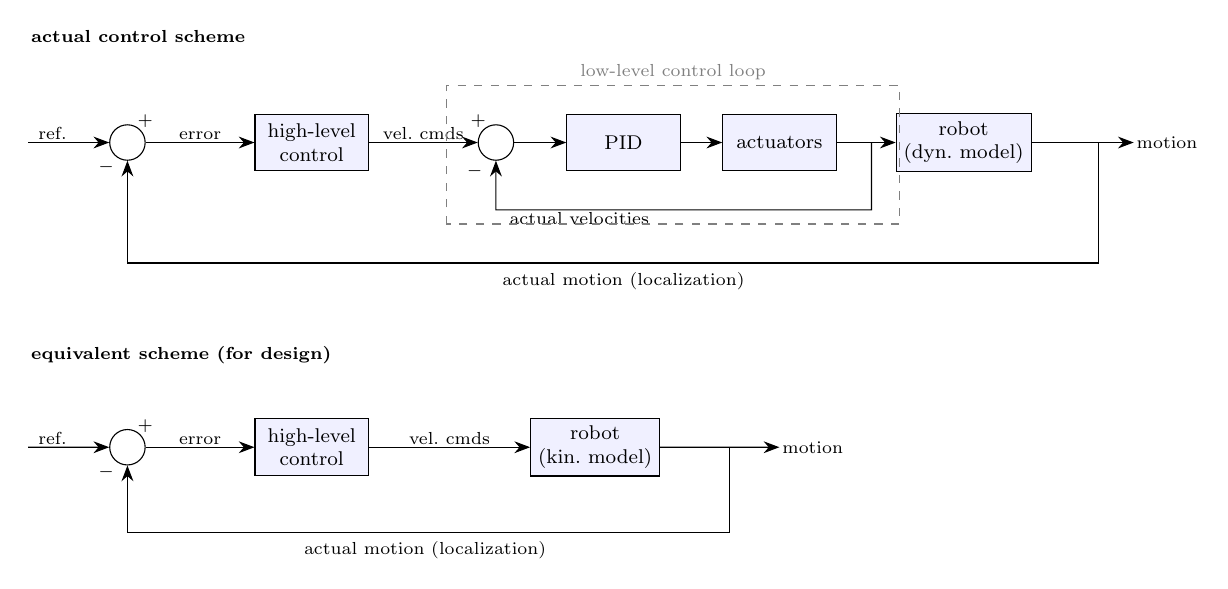
\begin{tikzpicture}[scale=0.9,transform shape]
\node[lab,anchor=west] at (-1.4,1.5) {\textbf{actual control scheme}};
\node[sm] (s1) at (0,0) {};
\node[blk] (hl1) at (2.6,0) {high-level\\control};
\node[sm] (s2) at (5.2,0) {};
\node[blk] (pid) at (7.0,0) {PID};
\node[blk] (act) at (9.2,0) {actuators};
\node[blk] (rb1) at (11.8,0) {robot\\(dyn.\ model)};
\draw[->] (-1.4,0) -- node[above,lab,pos=0.3]{ref.} (s1);
\draw[->] (s1) -- node[above,lab]{error} (hl1);
\draw[->] (hl1) -- node[above,lab]{vel.\ cmds} (s2);
\draw[->] (s2) -- (pid);
\draw[->] (pid) -- (act);
\draw[->] (act) -- (rb1);
\draw[->] (rb1) -- (14.2,0) node[right,lab]{motion};
\draw[->] (13.7,0) -- (13.7,-1.7) -- (0,-1.7) -- (s1.south);
\node[lab] at (7,-1.95) {actual motion (localization)};
\draw[->] (10.5,0) -- (10.5,-0.95) -- (5.2,-0.95) -- (s2.south);
\node[lab,anchor=north west] at (5.35,-0.95) {actual velocities};
\draw[dashed,gray] (4.5,-1.15) rectangle (10.9,0.8);
\node[lab,gray] at (7.7,1.0) {low-level control loop};
\node[lab] at (0.25,0.3) {$+$}; \node[lab] at (-0.3,-0.35) {$-$};
\node[lab] at (4.95,0.3) {$+$}; \node[lab] at (4.9,-0.4) {$-$};
% equivalent scheme
\node[lab,anchor=west] at (-1.4,-3.0) {\textbf{equivalent scheme (for design)}};
\node[sm] (t1) at (0,-4.3) {};
\node[blk] (hl2) at (2.6,-4.3) {high-level\\control};
\node[blk] (rb2) at (6.6,-4.3) {robot\\(kin.\ model)};
\draw[->] (-1.4,-4.3) -- node[above,lab,pos=0.3]{ref.} (t1);
\draw[->] (t1) -- node[above,lab]{error} (hl2);
\draw[->] (hl2) -- node[above,lab]{vel.\ cmds} (rb2);
\draw[->] (rb2) -- (9.2,-4.3) node[right,lab]{motion};
\draw[->] (8.5,-4.3) -- (8.5,-5.5) -- (0,-5.5) -- (t1.south);
\node[lab] at (4.2,-5.75) {actual motion (localization)};
\node[lab] at (0.25,-4.0) {$+$}; \node[lab] at (-0.3,-4.65) {$-$};
\end{tikzpicture}
\caption{Actual control scheme (top) and the equivalent scheme used for design (bottom): the fast low-level loops make the velocity commands act almost instantaneously, so the robot is seen as its kinematic model.}
\end{figure}

\begin{intuition}
Think of a driver and a car. The driver (high-level control) only decides ``how fast, how much steering''; the engine and steering servo (low-level loops) execute these requests much faster than the car moves on the road. So, for the purpose of planning the \emph{path-following behaviour}, we may forget engines and masses and say that the velocities we ask for are the velocities we get. This is exactly what makes the kinematic model~\eqref{eq:unicycle} a legitimate design model.
\end{intuition}

\subsection{Two motion control problems}

\begin{definition}[Trajectory tracking and posture regulation]
Two standard problems:
\begin{itemize}[nosep]
\item \emph{Trajectory tracking}: the robot must converge to (and then follow) a desired \emph{Cartesian trajectory} $\pd(t)$.
\item \emph{Posture regulation}: the robot must converge to a desired \emph{configuration} $\vect q_d=(x_d,y_d,\theta_d)$.
\end{itemize}
\end{definition}

Without loss of generality we consider the unicycle in what follows. Trajectory tracking is more relevant in practice, because moving along \emph{planned} trajectories reduces the risk of collision; on the other hand, posture regulation does not require planning.

\begin{figure}[H]
\centering
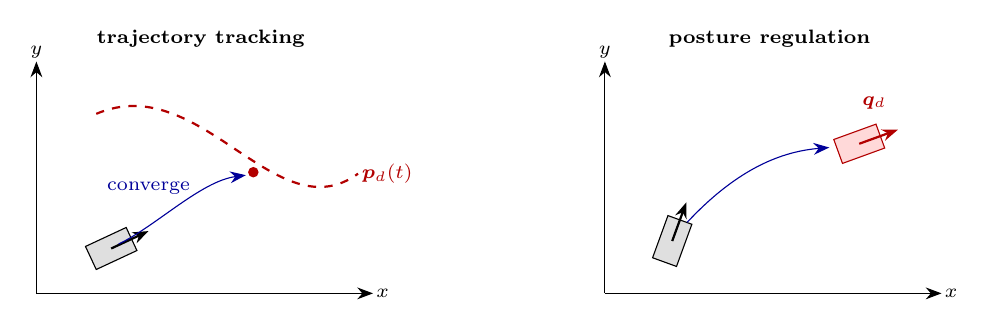
\begin{tikzpicture}[scale=0.95]
% trajectory tracking
\node[lab] at (2.2,3.4) {\textbf{trajectory tracking}};
\draw[->] (0,0) -- (4.5,0) node[right,lab]{$x$};
\draw[->] (0,0) -- (0,3.1) node[above,lab]{$y$};
\draw[red!70!black,thick,dashed] (0.8,2.4) .. controls (2.2,3.0) and (3.2,0.8) .. (4.3,1.6) node[right,lab,red!70!black]{$\pd(t)$};
\fill[red!70!black] (2.9,1.62) circle (2pt);
\begin{scope}[shift={(1.0,0.6)},rotate=25]
 \draw[fill=gray!25] (-0.3,-0.17) rectangle (0.3,0.17);
 \draw[->,thick] (0,0)--(0.55,0);
\end{scope}
\draw[->,blue!60!black] (1.1,0.66) .. controls (1.6,0.9) and (2.2,1.5) .. (2.8,1.58);
\node[lab,blue!60!black] at (1.5,1.4) {converge};
% posture regulation
\begin{scope}[shift={(7.6,0)}]
\node[lab] at (2.2,3.4) {\textbf{posture regulation}};
\draw[->] (0,0) -- (4.5,0) node[right,lab]{$x$};
\draw[->] (0,0) -- (0,3.1) node[above,lab]{$y$};
\begin{scope}[shift={(0.9,0.7)},rotate=70]
 \draw[fill=gray!25] (-0.3,-0.17) rectangle (0.3,0.17);
 \draw[->,thick] (0,0)--(0.55,0);
\end{scope}
\begin{scope}[shift={(3.4,2.0)},rotate=20]
 \draw[fill=red!15,draw=red!70!black] (-0.3,-0.17) rectangle (0.3,0.17);
 \draw[->,thick,red!70!black] (0,0)--(0.55,0);
\end{scope}
\node[lab,red!70!black] at (3.6,2.55) {$\vect q_d$};
\draw[->,blue!60!black] (1.1,0.95) .. controls (1.8,1.7) and (2.4,1.9) .. (3.0,1.95);
\end{scope}
\end{tikzpicture}
\caption{Tracking: follow a time-parametrized Cartesian path. Regulation: reach a final configuration (position \emph{and} orientation), with no prescribed intermediate motion.}
\end{figure}

%=====================================================================
\section{Trajectory Tracking: State Error Feedback \texorpdfstring{\emph{(slides 5--7)}}{(slides 5--7)}}
%=====================================================================

\subsection{Admissible trajectories and flatness}

The unicycle must track a Cartesian desired trajectory $(x_d(t),y_d(t))$ assumed to be \emph{admissible}.

\begin{definition}[Admissible Cartesian trajectory]
$(x_d(t),y_d(t))$ is admissible for the unicycle if there exist $\vd(t)$ and $\omd(t)$ such that
\[
\dot x_d=\vd\cos\theta_d,\qquad \dot y_d=\vd\sin\theta_d,\qquad \dot\theta_d=\omd .
\]
\end{definition}

The unicycle is \emph{differentially flat} with flat output $(x,y)$, so the whole desired state and input trajectory can be computed algebraically from $(x_d(t),y_d(t))$ and its derivatives.

\begin{proposition}[Flatness of the unicycle]\label{prop:flat}
Given an admissible $(x_d(t),y_d(t))$ with $\dot x_d^2+\dot y_d^2\neq0$,
\begin{align}
\theta_d(t)&=\atan\bigl(\dot y_d(t),\dot x_d(t)\bigr)+k\pi,\qquad k=0,1,\\
\vd(t)&=\pm\sqrt{\dot x_d^2(t)+\dot y_d^2(t)},\\
\omd(t)&=\frac{\ddot y_d(t)\dot x_d(t)-\ddot x_d(t)\dot y_d(t)}{\dot x_d^2(t)+\dot y_d^2(t)} .
\end{align}
\end{proposition}
\begin{proof}
Dividing the second kinematic equation by the first gives $\tan\theta_d=\dot y_d/\dot x_d$, hence the expression of $\theta_d$ (the choice of $k$ is the choice between forward and backward motion). Squaring and adding gives $\vd^2=\dot x_d^2+\dot y_d^2$, with the sign of $\vd$ matched to $k$: $\vd>0$ for $k=0$, $\vd<0$ for $k=1$. Finally $\omd=\dot\theta_d$, and differentiating $\atan(\dot y_d,\dot x_d)$ gives $(\ddot y_d\dot x_d-\ddot x_d\dot y_d)/(\dot x_d^2+\dot y_d^2)$, which is independent of $k$.
\end{proof}

Admissibility is guaranteed as long as $\dot y_d/\dot x_d$ is continuous in $t$, i.e.\ the tangent direction has no jumps (\emph{no sharp corners in time}).

\begin{intuition}
A car cannot move sideways: at every instant its velocity vector must point along its heading. So if you tell me \emph{where} the car must be at every time (the Cartesian curve), I already know \emph{how it must be oriented} (tangent to the curve), \emph{how fast} it goes (the speed along the curve) and \emph{how fast it must turn} (the curvature times the speed). There are no free choices left, apart from forward/backward ($k$). This is flatness: the Cartesian trajectory ``contains'' the full state and input history. The formulas also show why a trajectory that stops ($\dot x_d=\dot y_d=0$) is delicate: the heading is undefined there.
\end{intuition}

\subsection{The control scheme}

The desired state trajectory $\qd(t)=(x_d,y_d,\theta_d)$ is used to compute the \emph{state error}, from which the feedback action is generated; the nominal inputs $(\vd,\omd)$ are used as a \emph{feedforward} term.

\begin{figure}[H]
\centering
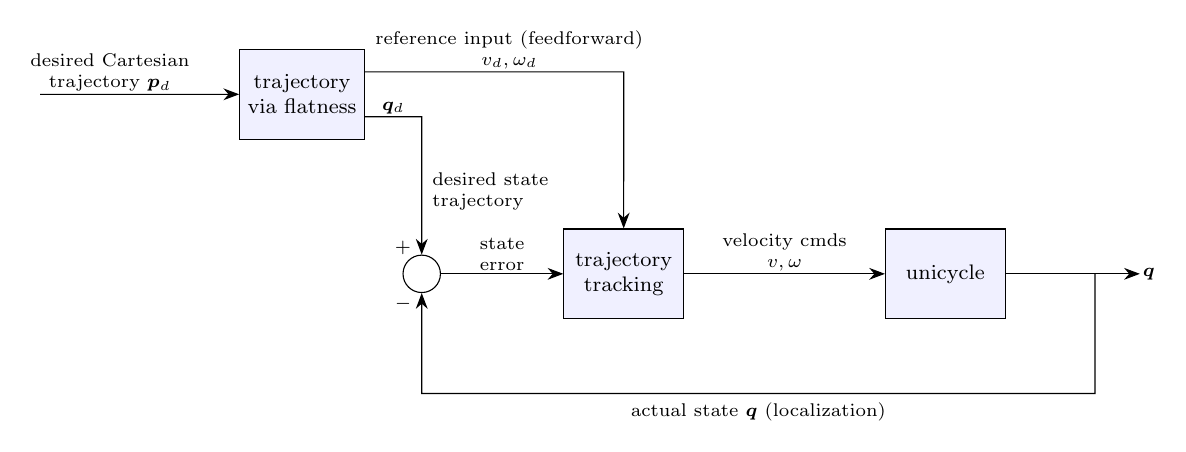
\begin{tikzpicture}[scale=0.95,transform shape]
\node[blk,minimum height=12mm] (fl) at (2.6,2.4) {trajectory\\via flatness};
\node[sm] (s) at (4.2,0) {};
\node[blk,minimum height=12mm] (tt) at (6.9,0) {trajectory\\tracking};
\node[blk,minimum height=12mm] (un) at (11.2,0) {unicycle};
\draw[->] (-0.9,2.4) -- node[above,lab,pos=0.35,align=center]{desired Cartesian\\trajectory $\pd$} (fl.west);
\draw[->] ($(fl.east)+(0,0.3)$) -- ++(0.4,0) coordinate (ff) -- node[above,lab,pos=0.5,align=center]{reference input (feedforward)\\$\vd,\omd$} (6.9,2.7) -- (tt.north);
\draw[->] ($(fl.east)+(0,-0.3)$) -- node[above,lab,pos=0.5]{$\qd$} (4.2,2.1) -- (s.north);
\node[lab,align=left,anchor=west] at (4.3,1.1) {desired state\\trajectory};
\draw[->] (s) -- node[above,lab,align=center]{state\\error} (tt);
\draw[->] (tt) -- node[above,lab,align=center]{velocity cmds\\$v,\omega$} (un);
\draw[->] (un) -- (13.8,0) node[right,lab]{$\vect q$};
\draw[->] (13.2,0) -- (13.2,-1.6) -- (4.2,-1.6) -- (s.south);
\node[lab] at (8.7,-1.85) {actual state $\vect q$ (localization)};
\node[lab] at (3.95,0.35) {$+$}; \node[lab] at (3.95,-0.4) {$-$};
\end{tikzpicture}
\caption{Trajectory tracking via state error feedback (block scheme): the desired Cartesian trajectory is turned into a desired state trajectory by flatness; the state error drives the tracking block, which also receives the nominal inputs $\vd,\omd$ as feedforward.}
\label{fig:state_basic}
\end{figure}

\subsection{Error coordinates and error dynamics}

The objective is to drive the state error to zero. Rather than $\qd-\vect q$ we use its \emph{rotated} version
\begin{equation}\label{eq:err}
\vect e=\begin{pmatrix}e_1\\e_2\\e_3\end{pmatrix}
=\begin{pmatrix}\cos\theta&\sin\theta&0\\-\sin\theta&\cos\theta&0\\0&0&1\end{pmatrix}
\begin{pmatrix}x_d-x\\y_d-y\\\theta_d-\theta\end{pmatrix}.
\end{equation}
$(e_1,e_2)$ is the Cartesian error $\vect e_p=\pd-\vect p$ expressed in a frame rotated by $\theta$, i.e.\ in the frame attached to the robot ($e_1$ along the sagittal axis, $e_2$ orthogonal to it), see Fig.~\ref{fig:errframe}.

\begin{figure}[H]
\centering
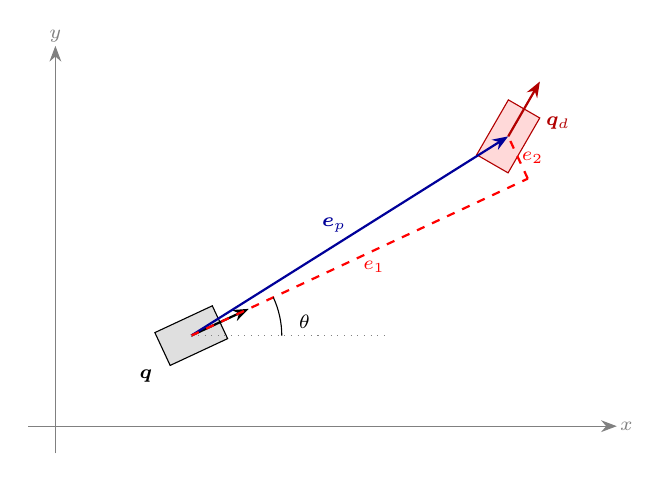
\begin{tikzpicture}[scale=1.15]
\draw[->,gray] (-0.3,0) -- (6.2,0) node[right,lab]{$x$};
\draw[->,gray] (0,-0.3) -- (0,4.2) node[above,lab]{$y$};
\coordinate (P) at (1.5,1);
\coordinate (D) at (5,3.2);
\coordinate (H) at (5.216,2.733);
\begin{scope}[shift={(P)},rotate=25]
 \draw[fill=gray!25] (-0.35,-0.2) rectangle (0.35,0.2);
 \draw[->,thick] (0,0)--(0.7,0);
\end{scope}
\begin{scope}[shift={(D)},rotate=60]
 \draw[fill=red!15,draw=red!70!black] (-0.35,-0.2) rectangle (0.35,0.2);
 \draw[->,thick,red!70!black] (0,0)--(0.7,0);
\end{scope}
\node[lab] at (1.0,0.55) {$\vect q$};
\node[lab,red!70!black] at (5.55,3.35) {$\qd$};
\draw[->,thick,blue!60!black] (P) -- (D) node[midway,above left,lab]{$\vect e_p$};
\draw[red,thick,dashed] (P) -- (H) node[midway,below right,lab,red]{$e_1$};
\draw[red,thick,dashed] (H) -- (D) node[midway,right,lab,red]{$e_2$};
\draw (1.5+1.0,1+0.0) arc (0:25:1.0) ;
\node[lab] at (2.75,1.15) {$\theta$};
\draw[gray,dotted] (P) -- ++(2.2,0);
\end{tikzpicture}
\caption{The rotated error: the Cartesian error $\vect e_p$ is decomposed along the robot's sagittal axis ($e_1$, ``how far ahead/behind is the target'') and orthogonally to it ($e_2$, ``how far to the side'').}
\label{fig:errframe}
\end{figure}

\begin{proposition}[Error dynamics]\label{prop:errdyn}
Along the trajectories of the unicycle~\eqref{eq:unicycle} and of the reference system, the error~\eqref{eq:err} obeys the \emph{nonlinear, time-varying} dynamics
\begin{align}
\dot e_1&=\vd\cos e_3-v+e_2\,\omega,\\
\dot e_2&=\vd\sin e_3-e_1\,\omega,\\
\dot e_3&=\omd-\omega .
\end{align}
\end{proposition}
\begin{proof}
Differentiate $e_1=\cos\theta(x_d-x)+\sin\theta(y_d-y)$:
\[
\dot e_1=\omega\bigl[-\sin\theta(x_d-x)+\cos\theta(y_d-y)\bigr]+\cos\theta(\dot x_d-\dot x)+\sin\theta(\dot y_d-\dot y)
=\omega e_2+\vd\cos(\theta_d-\theta)-v ,
\]
where we used $\dot x_d=\vd\cos\theta_d$, $\dot y_d=\vd\sin\theta_d$, $\dot x=v\cos\theta$, $\dot y=v\sin\theta$ and $\cos\theta\cos\theta_d+\sin\theta\sin\theta_d=\cos(\theta_d-\theta)$. The computation of $\dot e_2$ is analogous, using $-\sin\theta\cos\theta_d+\cos\theta\sin\theta_d=\sin(\theta_d-\theta)$, and $\dot e_3=\omd-\omega$ is immediate.
\end{proof}

\begin{intuition}
The term $e_2\omega$ in $\dot e_1$ (and $-e_1\omega$ in $\dot e_2$) is the price of using a \emph{rotating} frame: when the robot turns, the frame turns with it and the components of a fixed error vector mix, exactly as the components of a fixed arrow rotate when you spin your coordinate axes. In exchange, the other terms are very readable: $\vd\cos e_3-v$ says ``if I drive slower than the reference speed (projected on my heading), the target runs away from me along $e_1$''.
\end{intuition}

%=====================================================================
\section{Approximate Linearization: Brush-up \texorpdfstring{\emph{(slides 8--9)}}{(slides 8--9)}}
%=====================================================================

The idea: to stabilize a nonlinear system at an equilibrium, stabilize its \emph{approximate linearization} around it. Consider
\[
\dot{\vect x}=\vect\eta(\vect x,\vect u)=\vect f(\vect x)+\vect G(\vect x)\vect u,\qquad \vect x\in\R^n,\ \vect u\in\R^m,
\]
and assume (w.l.o.g.) that the origin is the desired \emph{unforced} equilibrium: $\vect\eta(\vect 0,\vect 0)=\vect 0$, or equivalently $\vect f(\vect 0)=\vect 0$. The Taylor expansion of $\vect\eta$ around $\vect x=\vect 0,\vect u=\vect 0$ gives
\[
\vect\eta(\vect x,\vect u)\approx\cancel{\vect\eta(\vect 0,\vect 0)}+\left.\frac{\partial\vect\eta}{\partial\vect x}\right|_{\substack{\vect x=\vect 0\\ \vect u=\vect 0}}\vect x+\left.\frac{\partial\vect\eta}{\partial\vect u}\right|_{\substack{\vect x=\vect 0\\ \vect u=\vect 0}}\vect u .
\]
The \emph{approximate linearization} at the origin is then
\[
\dot{\vect x}=\vect A\vect x+\vect B\vect u,\qquad \vect A=\left.\frac{\partial\vect\eta}{\partial\vect x}\right|_{\vect 0,\vect 0},\quad \vect B=\left.\frac{\partial\vect\eta}{\partial\vect u}\right|_{\vect 0,\vect 0}.
\]
Let $\vect u=\vect K\vect x$, so that $\dot{\vect x}=(\vect A+\vect B\vect K)\vect x$. If $\vect K$ is chosen so that $\vect A+\vect B\vect K$ is \emph{Hurwitz} (certainly possible if $(\vect A,\vect B)$ is controllable), the approximate linearization is asymptotically stable.

\begin{theorem}[Lyapunov indirect method]\label{thm:indirect}
If $\vect A+\vect B\vect K$ is Hurwitz, the origin is a \emph{locally} asymptotically stable equilibrium of the nonlinear closed-loop system $\dot{\vect x}=\vect\eta(\vect x,\vect K\vect x)$. (If $\vect A+\vect B\vect K$ has an eigenvalue with positive real part the origin is unstable; if the eigenvalues are only marginally stable, the linearization is inconclusive.)
\end{theorem}

\begin{intuition}
Zoom in enough on any smooth function and it looks like a straight line (here, a linear map). If the linear caricature of the system is stable, then close enough to the equilibrium the true system behaves like it and is stable too. The word \emph{local} is essential: the linear model says nothing about what happens far away, where the curvature (the neglected nonlinear terms) matters. That is exactly why this method will only give local guarantees for the unicycle.
\end{intuition}

%=====================================================================
\section{Tracking via Approximate Linearization \texorpdfstring{\emph{(slides 10--16)}}{(slides 10--16)}}
%=====================================================================

\subsection{Input transformation: making the origin an equilibrium}

Apply the approximate linearization approach to the error dynamics of Proposition~\ref{prop:errdyn}. In that form the origin is \emph{not} an unforced equilibrium (even with $\vect e=\vect 0$, the terms $\vd-v$ and $\omd-\omega$ would not vanish unless the inputs equal the reference). This is rectified by the invertible \emph{input transformation}
\begin{equation}\label{eq:inputtransf}
w_1=\vd\cos e_3-v,\qquad w_2=\omd-\omega .
\end{equation}
The error dynamics $\dot{\vect e}=\vect\eta(\vect e,\vect w)$ becomes
\begin{equation}\label{eq:errfG}
\dot{\vect e}=\underbrace{\begin{pmatrix}\omd e_2\\-\omd e_1+\vd\sin e_3\\0\end{pmatrix}}_{\vect f(\vect e)}
+\underbrace{\begin{pmatrix}1&-e_2\\0&e_1\\0&1\end{pmatrix}}_{\vect G(\vect e)}\begin{pmatrix}w_1\\w_2\end{pmatrix},
\end{equation}
which is at rest when $\vect e=\vect 0,\vect w=\vect 0$, i.e.\ $\vect\eta(\vect 0,\vect 0)=\vect 0$. Both the drift and the input term are nonlinear; in general the drift is also time-varying (through $\vd(t),\omd(t)$).

\begin{intuition}
The new inputs $\vect w$ are simply ``\emph{how far the actual velocities deviate from what is needed to keep the error at rest}''. $w_1=0$ means we drive at the speed that makes $e_1$ stand still; $w_2=0$ means we turn at the reference rate. Feedback will generate $\vect w$ from the error; the actual commands $(v,\omega)$ are recovered afterwards by inverting~\eqref{eq:inputtransf}. So the feedforward $(\vd,\omd)$ is automatically included.
\end{intuition}

\subsection{The linear approximation}

One easily finds
\[
\frac{\partial\vect\eta}{\partial\vect e}=\begin{pmatrix}0&\omd-w_2&0\\-\omd+w_2&0&\vd\cos e_3\\0&0&0\end{pmatrix},\qquad
\frac{\partial\vect\eta}{\partial\vect w}=\begin{pmatrix}1&-e_2\\0&e_1\\0&1\end{pmatrix}.
\]
Letting $\vect e=\vect 0,\vect w=\vect 0$ gives
\[
\vect A(t)=\begin{pmatrix}0&\omd&0\\-\omd&0&\vd\\0&0&0\end{pmatrix},\qquad
\vect B=\begin{pmatrix}1&0\\0&0\\0&1\end{pmatrix}.
\]
Note that $\vect A$ is actually $\vect A(t)$ because of the dependence of $\vd$ and $\omd$ on time $\Rightarrow$ the linear approximation is still a \emph{time-varying} system!

Define the \emph{linear} feedback
\[
\vect w=\begin{pmatrix}w_1\\w_2\end{pmatrix}=\begin{pmatrix}-k_1&0&0\\0&-k_2&-k_3\end{pmatrix}\begin{pmatrix}e_1\\e_2\\e_3\end{pmatrix}=\vect K\vect e .
\]
The closed-loop error dynamics is still time-varying:
\begin{equation}\label{eq:Acl}
\dot{\vect e}=(\vect A(t)+\vect B\vect K)\vect e=\Acl(t)\vect e=\begin{pmatrix}-k_1&\omd&0\\-\omd&0&\vd\\0&-k_2&-k_3\end{pmatrix}\vect e .
\end{equation}

\subsection{Gain tuning}

\begin{proposition}[Pole placement for the frozen system]\label{prop:poles}
Letting
\[
k_1=k_3=2\zeta a,\qquad k_2=\frac{a^2-\omd^2}{\vd},\qquad a>0,\ \zeta\in(0,1),
\]
the characteristic polynomial of $\Acl(t)$ becomes time-invariant and Hurwitz:
\[
p(\lambda)=(\lambda+2\zeta a)(\lambda^2+2\zeta a\lambda+a^2).
\]
\end{proposition}
\begin{proof}
Expanding $\det(\lambda\vect I-\Acl)$ along the first row,
\[
\det\begin{pmatrix}\lambda+k_1&-\omd&0\\\omd&\lambda&-\vd\\0&k_2&\lambda+k_3\end{pmatrix}
=(\lambda+k_1)\bigl(\lambda^2+k_3\lambda+\vd k_2\bigr)+\omd^2(\lambda+k_3).
\]
With $k_1=k_3=2\zeta a$ and $\vd k_2=a^2-\omd^2$ this becomes $(\lambda+2\zeta a)\bigl(\lambda^2+2\zeta a\lambda+a^2-\omd^2\bigr)+\omd^2(\lambda+2\zeta a)=(\lambda+2\zeta a)(\lambda^2+2\zeta a\lambda+a^2)$.
\end{proof}

The polynomial has \emph{one real negative eigenvalue} $-2\zeta a$ and \emph{two complex eigenvalues with damping $\zeta$ and natural frequency $a$}, $\lambda=-\zeta a\pm ja\sqrt{1-\zeta^2}$.

\begin{figure}[H]
\centering
\begin{tikzpicture}[scale=0.95]
\draw[->] (-4.2,0) -- (1.2,0) node[right,lab]{$\mathrm{Re}$};
\draw[->] (0,-2.7) -- (0,2.7) node[above,lab]{$\mathrm{Im}$};
\draw[dashed,gray] (0,0) circle (2);
\node[lab,gray] at (0.55,-2.15) {$|\lambda|=a$};
\fill[red!70!black] (-2.8,0) circle (2.2pt) node[above=3pt,lab,red!70!black]{$-2\zeta a$};
\fill[red!70!black] (-1.4,1.428) circle (2.2pt);
\fill[red!70!black] (-1.4,-1.428) circle (2.2pt);
\draw[red!70!black,dotted] (0,0) -- (-1.4,1.428);
\draw (-0.9,0) arc (180:134.4:0.9);
\node[lab] at (-1.15,0.55) {$\varphi$};
\node[lab,red!70!black,right] at (-1.3,1.75) {$\cos\varphi=\zeta$};
\end{tikzpicture}
\caption{Closed-loop eigenvalues for $a=2,\ \zeta=0.7$: a real pole at $-2\zeta a$ and a complex pair on the circle of radius $a$ with damping $\zeta$ (the angle $\varphi$ from the negative real axis satisfies $\cos\varphi=\zeta$).}
\end{figure}

\begin{intuition}
The two gains $k_1,k_3$ are chosen equal to the damping term and $k_2$ absorbs the (time-varying) reference velocities $\vd,\omd$. The trick is ``gain scheduling'': we \emph{re-compute $k_2$ at every instant} so that the frozen-time eigenvalues stay at the same place. The designer then simply chooses the response speed $a$ and damping $\zeta$, as for a second-order system. Note the price: $k_2=(a^2-\omd^2)/\vd\to\infty$ as $\vd\to0$.
\end{intuition}

\begin{remark}[Caveat]
Having time-invariant, Hurwitz \emph{frozen-time} eigenvalues does \emph{not} guarantee asymptotic stability of a time-varying system. Stability is guaranteed only if $\vd$ and $\omd$ are constant ($\Rightarrow$ $\Acl$ constant), i.e.\ for rectilinear and circular reference trajectories, and then Theorem~\ref{thm:indirect} gives only \emph{local} asymptotic stability, not global.
\end{remark}

\subsection{Actual inputs, limitations and a global version}

The actual velocity inputs $(v,\omega)$ are obtained by plugging the feedback controls $w_1,w_2$ in the input transformation~\eqref{eq:inputtransf}:
\begin{equation}\label{eq:actualinputs}
v=\vd\cos e_3-w_1=\vd\cos e_3+k_1e_1,\qquad
\omega=\omd-w_2=\omd+k_2e_2+k_3e_3 .
\end{equation}
Two remarks:
\begin{itemize}[nosep]
\item $(v,\omega)\to(\vd,\omd)$ as $\vect e\to\vect 0$: the controller reduces to pure feedforward.
\item $k_2\to\infty$ as $\vd\to0$, so this controller can only be used with \emph{persistent} Cartesian trajectories (stops are not allowed).
\end{itemize}

\begin{theorem}[Global stability via a nonlinear version]\label{thm:nonlin}
Global asymptotic stability of $\vect e=\vect 0$ is obtained by the nonlinear feedback
\begin{align}
w_1&=-k_1(\vd,\omd)\,e_1,\\
w_2&=-k_2\,\vd\,\frac{\sin e_3}{e_3}\,e_2-k_3(\vd,\omd)\,e_3,
\end{align}
if $k_1,k_3$ are bounded, positive, with bounded derivatives (and $k_2>0$ constant), and $\vd,\omd$ are bounded, with $\vd$ not vanishing asymptotically.
\end{theorem}

\begin{intuition}
In the linearized controller the term $k_2\vd e_2$ is linear in $e_3$-space, i.e.\ it approximates $\sin e_3$ by $e_3$. The nonlinear version keeps $\sin e_3/e_3$, which is bounded (between $-0.22$ and $1$ for all $e_3$): large heading errors can no longer produce unreasonably large commands, and a Lyapunov argument (not repeated here) works globally. The structure is the same, and when $e_3$ is small the two controllers coincide.
\end{intuition}

\begin{algorithm}[Tracking via state error feedback and approximate linearization]
At each control instant:
\begin{enumerate}[nosep]
\item from $(x_d,y_d)$ compute $\theta_d,\vd,\omd$ via flatness (Prop.~\ref{prop:flat});
\item read $(x,y,\theta)$ from localization and compute $\vect e$ with~\eqref{eq:err};
\item compute gains $k_1=k_3=2\zeta a$, $k_2=(a^2-\omd^2)/\vd$;
\item set $v=\vd\cos e_3+k_1e_1$ and $\omega=\omd+k_2e_2+k_3e_3$.
\end{enumerate}
\end{algorithm}

\begin{figure}[H]
\centering
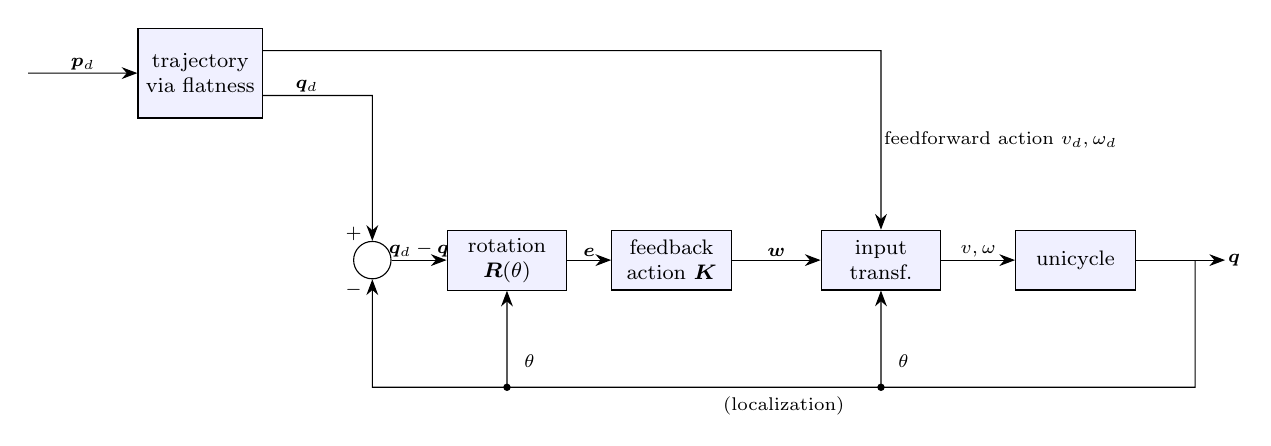
\begin{tikzpicture}[scale=0.95,transform shape]
\node[blk,minimum height=12mm] (fl) at (1.7,2.5) {trajectory\\via flatness};
\node[sm] (s) at (4.0,0) {};
\node[blk] (rot) at (5.8,0) {rotation\\$\vect R(\theta)$};
\node[blk] (K) at (8.0,0) {feedback\\action $\vect K$};
\node[blk] (it) at (10.8,0) {input\\transf.};
\node[blk] (un) at (13.4,0) {unicycle};
\draw[->] (-0.6,2.5) -- node[above,lab]{$\pd$} (fl.west);
\draw[->] ($(fl.east)+(0,-0.3)$) -- node[above,lab,pos=0.4]{$\qd$} (4.0,2.2) -- (s.north);
\draw[->] ($(fl.east)+(0,0.3)$) -- (10.8,2.8) -- node[right,lab,pos=0.5]{feedforward action $\vd,\omd$} (it.north);
\draw[->] (s) -- node[above,lab]{$\qd-\vect q$} (rot);
\draw[->] (rot) -- node[above,lab]{$\vect e$} (K);
\draw[->] (K) -- node[above,lab]{$\vect w$} (it);
\draw[->] (it) -- node[above,lab]{$v,\omega$} (un);
\draw[->] (un) -- (15.4,0) node[right,lab]{$\vect q$};
\draw[->] (15.0,0) -- (15.0,-1.7) -- (4.0,-1.7) -- (s.south);
\node[lab] at (9.5,-1.95) {(localization)};
\draw[->] (5.8,-1.7) -- (rot.south);
\draw[->] (10.8,-1.7) -- (it.south);
\node[dot] at (5.8,-1.7) {}; \node[dot] at (10.8,-1.7) {};
\node[lab] at (6.1,-1.35) {$\theta$}; \node[lab] at (11.1,-1.35) {$\theta$};
\node[lab] at (3.75,0.35) {$+$}; \node[lab] at (3.75,-0.4) {$-$};
\end{tikzpicture}
\caption{Detailed version of Fig.~\ref{fig:state_basic} for approximate linearization: a static controller on the rotated state error, with feedforward $\vd,\omd$ added through the input transformation.}
\label{fig:state_scheme}
\end{figure}

The final scheme (Fig.~\ref{fig:state_scheme}) is a \emph{static} controller based on the state error; it needs $\vd,\omd$, and needs $\theta$ both for the error rotation and for the input transformation.

%=====================================================================
\section{Trajectory Tracking: Output Error Feedback \emph{(slide 17)}}
%=====================================================================

Another approach: develop the feedback action from the \emph{output (Cartesian) error} only, \emph{without} computing a desired state trajectory, using as \emph{feedforward} term the velocity $\dot{\pd}$ along the reference trajectory.

\begin{figure}[H]
\centering
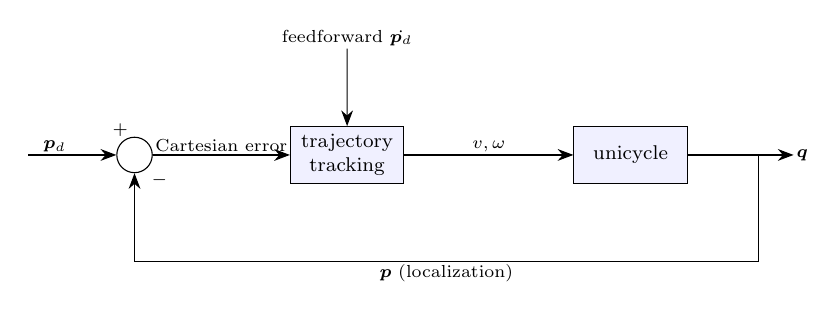
\begin{tikzpicture}[scale=0.9,transform shape]
\node[sm] (s) at (0,0) {};
\node[blk] (tt) at (3,0) {trajectory\\tracking};
\node[blk] (un) at (7,0) {unicycle};
\draw[->] (-1.5,0) -- node[above,lab,pos=0.3]{$\pd$} (s);
\draw[->] (s) -- node[above,lab]{Cartesian error} (tt);
\draw[->] (tt) -- node[above,lab]{$v,\omega$} (un);
\draw[->] (un) -- (9.3,0) node[right,lab]{$\vect q$};
\draw[->] (3,1.5) node[above,lab]{feedforward $\dot{\pd}$} -- (tt.north);
\draw[->] (8.8,0) -- (8.8,-1.5) -- (0,-1.5) node[pos=0.5,below,lab]{$\vect p$ (localization)} -- (s.south);
\node[lab] at (-0.2,0.35) {$+$}; \node[lab] at (0.35,-0.35) {$-$};
\end{tikzpicture}
\caption{Output error feedback: only the Cartesian error is fed back.}
\end{figure}

The difficulty is that the unicycle has two inputs and, if only $(x,y)$ is to be controlled, a standard linearization-by-feedback argument must be adapted. The next section recalls the tool, and the following ones apply it in two different ways.

%=====================================================================
\section{Exact I/O Linearization: Brush-up \texorpdfstring{\emph{(slides 18--19)}}{(slides 18--19)}}
%=====================================================================

Consider a driftless nonlinear system with as many outputs as inputs:
\[
\dot{\vect x}=\vect G(\vect x)\vect u,\qquad \vect y=\vect h(\vect x),\qquad \vect x\in\R^n,\ \vect u\in\R^m,\ \vect y\in\R^m .
\]
Since
\[
\dot{\vect y}=\frac{\partial\vect h}{\partial\vect x}\dot{\vect x}=\underbrace{\frac{\partial\vect h}{\partial\vect x}\vect G(\vect x)}_{\vect T(\vect x)}\vect u=\vect T(\vect x)\vect u,
\]
we call $\vect T$ ($m\times m$) the \emph{decoupling matrix}.

\begin{proposition}[Exact input--output linearization]\label{prop:io}
If $\vect T(\vect x)$ is invertible, the \emph{linearizing feedback} $\vect u=\vect T^{-1}(\vect x)\vect w$ yields
\[
\dot{\vect y}=\vect T(\vect x)\vect T^{-1}(\vect x)\vect w=\vect w,
\]
i.e.\ an exactly linear (and decoupled) map between the new inputs $\vect w$ and the time derivative of the outputs. Given a reference output $\vect y_d(t)$, the output error $\vect e=\vect y_d-\vect y$ has dynamics $\dot{\vect e}=\dot{\vect y}_d-\vect w$; the law $\vect w=\dot{\vect y}_d+\vect K\vect e$ (feedforward + proportional feedback) gives $\dot{\vect e}=-\vect K\vect e$, i.e.\ \emph{global exponential stability} of $\vect e=\vect 0$ provided that the eigenvalues of $\vect K$ are in the right half-plane. The final control law is
\begin{equation}\label{eq:iolaw}
\vect u=\vect T^{-1}(\vect x)\bigl(\dot{\vect y}_d+\vect K\vect e\bigr).
\end{equation}
\end{proposition}

\begin{figure}[H]
\centering
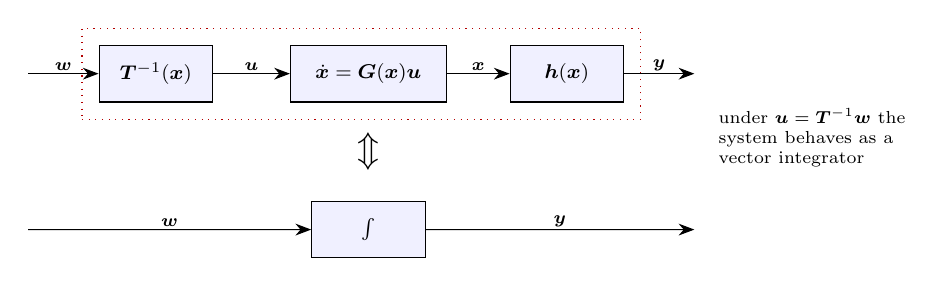
\begin{tikzpicture}[scale=0.9,transform shape]
\node[blk] (T) at (1.6,0) {$\vect T^{-1}(\vect x)$};
\node[blk,minimum width=22mm] (sys) at (4.6,0) {$\dot{\vect x}=\vect G(\vect x)\vect u$};
\node[blk] (h) at (7.4,0) {$\vect h(\vect x)$};
\draw[->] (-0.2,0) -- node[above,lab]{$\vect w$} (T);
\draw[->] (T) -- node[above,lab]{$\vect u$} (sys);
\draw[->] (sys) -- node[above,lab]{$\vect x$} (h);
\draw[->] (h) -- node[above,lab]{$\vect y$} (9.2,0);
\node[draw,dotted,red!70!black,fit=(T)(sys)(h),inner sep=6pt] (box) {};
\node[blk] (int) at (4.6,-2.2) {$\int$};
\draw[->] (-0.2,-2.2) -- node[above,lab]{$\vect w$} (int);
\draw[->] (int) -- node[above,lab]{$\vect y$} (9.2,-2.2);
\node[font=\Large] at (4.6,-1.1) {$\Updownarrow$};
\node[lab,align=left,anchor=west] at (9.5,-0.9) {under $\vect u=\vect T^{-1}\vect w$ the\\system behaves as a\\vector integrator};
\end{tikzpicture}
\caption{Exact input--output linearization: the dotted block, seen from $\vect w$ to $\vect y$, is just a bank of integrators.}
\end{figure}

\begin{intuition}
Imagine a robot arm where you want the hand velocity $\dot{\vect y}$ and you can command joint velocities $\vect u$ through a Jacobian-like matrix $\vect T(\vect x)$. If you multiply the desired hand velocity by the inverse Jacobian, the hand does exactly what you wanted, and the plant ``disappears'': what remains is $\dot y=w$, the simplest system in the world. Tracking becomes trivial: ask for the reference velocity plus a correction proportional to the error. Everything hinges on $\vect T$ being \emph{invertible}.
\end{intuition}

%=====================================================================
\section{Tracking via I/O Linearization: Static Feedback \texorpdfstring{\emph{(slides 20--24)}}{(slides 20--24)}}
%=====================================================================

\subsection{The singularity for the output $(x,y)$}

Let us apply exact i/o linearization to the unicycle with output $(x,y)$. However, the decoupling matrix is
\[
\begin{pmatrix}\dot x\\\dot y\end{pmatrix}=\begin{pmatrix}\cos\theta&0\\\sin\theta&0\end{pmatrix}\begin{pmatrix}v\\\omega\end{pmatrix},
\]
which is \emph{singular} (its second column is zero): $\omega$ does not appear in the first derivative of $(x,y)$. Hence exact input--output linearization is \emph{not possible} for the output $(x,y)$ by static feedback.

\begin{intuition}
At the contact point of the wheel, turning in place does not move the point. The steering command is invisible at the level of positions, so we cannot ``invert'' the map. The cure is to look at a point that \emph{does} move when you steer.
\end{intuition}

\subsection{Displacing the output to a point $B$}

Solution: \emph{change slightly the output} so that the new input--output map is invertible. In particular, displace the output from the contact point of the wheel to a point $B$ along the sagittal axis, at distance $b$:
\[
x_B=x+b\cos\theta,\qquad y_B=y+b\sin\theta .
\]

\begin{figure}[H]
\centering
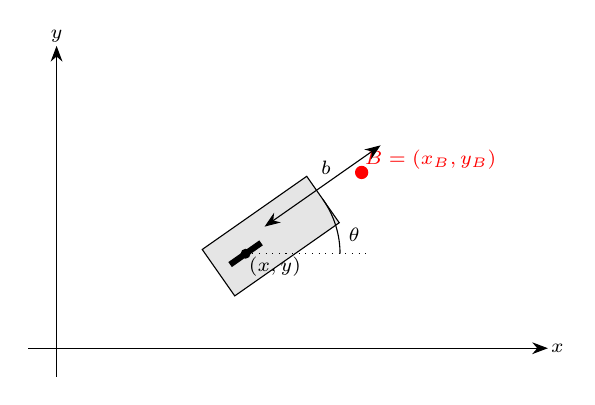
\begin{tikzpicture}[scale=1.2]
\draw[->] (-0.3,0) -- (5.2,0) node[right,lab]{$x$};
\draw[->] (0,-0.3) -- (0,3.2) node[above,lab]{$y$};
\coordinate (P) at (2,1);
\coordinate (B) at (3.228,1.860);
\begin{scope}[shift={(P)},rotate=35]
 \draw[fill=gray!20] (-0.35,-0.3) rectangle (1.0,0.3);
 \draw[line width=2.2pt] (-0.2,0)--(0.2,0);
 \node[rotate=0] at (0,0) {};
\end{scope}
\fill (P) circle (1.5pt) node[below right,lab]{$(x,y)$};
\fill[red] (B) circle (2pt) node[above right,lab,red]{$B=(x_B,y_B)$};
\draw[<->] ($(P)+(-35+90:0.35)$) -- node[above left,lab,pos=0.6]{$b$} ($(B)+(-35+90:0.35)$);
\draw[dotted] (P) -- ++(1.3,0);
\draw (3.0,1.0) arc (0:35:1.0);
\node[lab] at (3.15,1.2) {$\theta$};
\end{tikzpicture}
\caption{Point $B$ at distance $b$ ahead of the wheel contact point along the sagittal axis.}
\end{figure}

Differentiating with respect to time,
\[
\begin{pmatrix}\dot x_B\\\dot y_B\end{pmatrix}=\underbrace{\begin{pmatrix}\cos\theta&-b\sin\theta\\\sin\theta&b\cos\theta\end{pmatrix}}_{\vect T(\theta),\ \det=b}\begin{pmatrix}v\\\omega\end{pmatrix}.
\]
If $b\neq0$ we may set
\begin{equation}\label{eq:Tinv}
\begin{pmatrix}v\\\omega\end{pmatrix}=\vect T^{-1}(\theta)\begin{pmatrix}w_1\\w_2\end{pmatrix}=\begin{pmatrix}\cos\theta&\sin\theta\\-\sin\theta/b&\cos\theta/b\end{pmatrix}\begin{pmatrix}w_1\\w_2\end{pmatrix},
\end{equation}
obtaining the input--output linearized system
\[
\dot x_B=w_1,\qquad \dot y_B=w_2,\qquad \dot\theta=\frac{w_2\cos\theta-w_1\sin\theta}{b}.
\]
(The third equation is the part of the dynamics that is \emph{not} seen from the output.)

We achieve \emph{global exponential convergence} of $(x_B,y_B)$ to the desired trajectory by letting
\[
w_1=\dot x_d+k_x(x_d-x_B),\qquad w_2=\dot y_d+k_y(y_d-y_B),\qquad k_x,k_y>0 .
\]

\begin{intuition}
Hold a broom by its middle and push the handle sideways: the bristle end ($B$) moves sideways even if the hand does not. In the same way, a point ahead of the axle \emph{moves laterally when the robot steers}, so both of its velocity components can be commanded; $b$ is the lever arm, and $\det\vect T=b$ tells us that the shorter the lever arm, the more delicate the inversion (the $1/b$ in the second row of~\eqref{eq:Tinv} amplifies the steering command).
\end{intuition}

\subsection{What happens to $\theta$: zero dynamics}

The orientation $\theta$ is \emph{not} controlled by this scheme, which is based on output error feedback: there is a \emph{zero dynamics}. Still, it must evolve as dictated by flatness. The next result makes this precise.

\begin{proposition}[Zero dynamics]\label{prop:zerodyn}
Suppose $B$ tracks the reference exactly, so $w_1=\dot x_d$, $w_2=\dot y_d$. Writing $\dot{\pd}=|\dot{\pd}|(\cos\varphi,\sin\varphi)$ and $\delta=\theta-\varphi$,
\[
\dot\delta=-\frac{|\dot{\pd}|}{b}\sin\delta+(\text{terms in }\dot\varphi),
\]
and for the case $\varphi=\text{const}$ (straight reference) $\delta=0$ is exponentially stable if $|\dot{\pd}|>0$ and $b>0$, while $\delta=\pi$ is unstable.
\end{proposition}
\begin{proof}
Substitute $w_1,w_2$ in $\dot\theta$: $\dot\theta=\bigl(\dot y_d\cos\theta-\dot x_d\sin\theta\bigr)/b=\frac{|\dot{\pd}|}{b}\sin(\varphi-\theta)$. Subtracting $\dot\varphi$ gives the claim; linearization at $\delta=0$ gives $\dot\delta\simeq-(|\dot{\pd}|/b)\delta$, at $\delta=\pi$ it gives $+(|\dot{\pd}|/b)\delta'$.
\end{proof}

\begin{figure}[H]
\centering
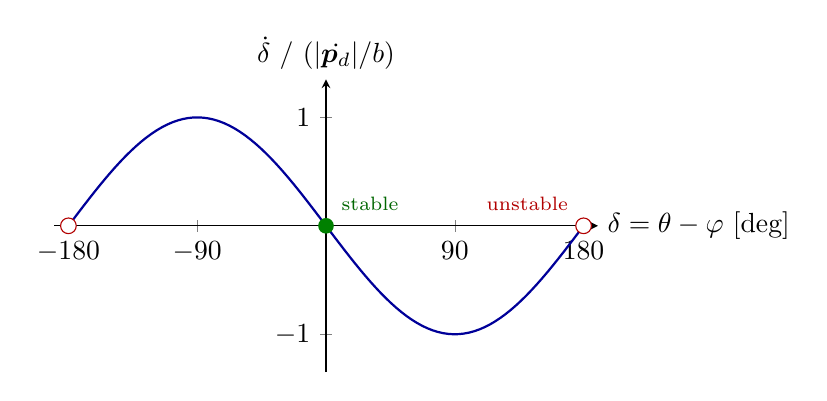
\begin{tikzpicture}
\begin{axis}[width=0.7\textwidth,height=5.3cm,xlabel={$\delta=\theta-\varphi$ [deg]},ylabel={$\dot\delta\ /\ (|\dot{\pd}|/b)$},
  xmin=-190,xmax=190,ymin=-1.35,ymax=1.35,xtick={-180,-90,0,90,180},axis lines=middle,
  every axis x label/.style={at={(current axis.right of origin)},anchor=west},
  every axis y label/.style={at={(current axis.above origin)},anchor=south},
  samples=100,domain=-180:180]
\addplot[thick,blue!60!black]{-sin(x)};
\node[circle,fill=green!50!black,inner sep=2pt,label={[font=\scriptsize,green!40!black]above right:stable}] at (axis cs:0,0) {};
\node[circle,draw=red!70!black,fill=white,inner sep=2pt,label={[font=\scriptsize,red!70!black]above left:unstable}] at (axis cs:180,0) {};
\node[circle,draw=red!70!black,fill=white,inner sep=2pt] at (axis cs:-180,0) {};
\end{axis}
\end{tikzpicture}
\caption{Phase line of the zero dynamics (straight reference): the robot's orientation relaxes to the direction of motion of $B$.}
\end{figure}

\begin{intuition}
It is like towing a shopping cart by its front end: if you pull $B$ along a path, the cart (robot body) lines up behind the pulling point and follows the tangent of the path. Aligned forward ($\delta=0$) is stable. Driving \emph{backwards}, with the body ahead of the pulled point, is unstable: the same reason a cart pushed from behind jackknifes. This is why the scheme is used with forward motion only.
\end{intuition}

\subsection{Properties and block scheme}

The desired trajectory for $B$ can be \emph{arbitrary}; in particular, \emph{square corners may be included}, since no desired heading has to be computed.

\begin{figure}[H]
\centering
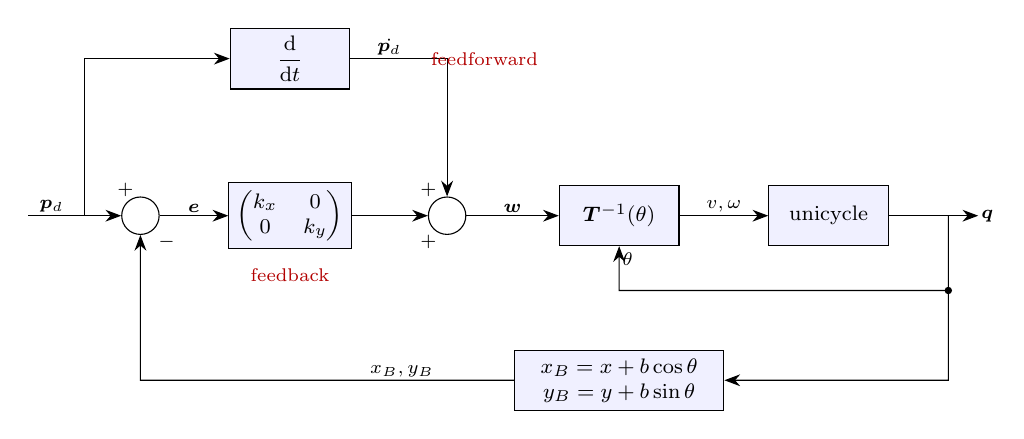
\begin{tikzpicture}[scale=0.95,transform shape]
\node[sm] (s1) at (0,0) {};
\node[blk,minimum width=14mm] (K) at (2.0,0) {$\begin{pmatrix}k_x&0\\0&k_y\end{pmatrix}$};
\node[sm] (s2) at (4.1,0) {};
\node[blk] (T) at (6.4,0) {$\vect T^{-1}(\theta)$};
\node[blk] (un) at (9.2,0) {unicycle};
\node[blk] (d) at (2.0,2.1) {$\dfrac{\dd}{\dd t}$};
\node[blk,minimum width=28mm] (out) at (6.4,-2.2) {$x_B=x+b\cos\theta$\\$y_B=y+b\sin\theta$};
\draw[->] (-1.5,0) -- node[above,lab,pos=0.25]{$\pd$} (s1);
\draw[->] (-0.75,0) |- (d.west);
\draw[->] (s1) -- node[above,lab]{$\vect e$} (K);
\draw[->] (K) -- (s2);
\draw[->] (d.east) -| node[above,lab,pos=0.2]{$\dot{\pd}$} (s2.north);
\draw[->] (s2) -- node[above,lab]{$\vect w$} (T);
\draw[->] (T) -- node[above,lab]{$v,\omega$} (un);
\draw[->] (un) -- (11.2,0) node[right,lab]{$\vect q$};
\draw[->] (10.8,0) -- (10.8,-2.2) -- (out.east);
\draw[->] (out.west) -- node[above,lab,pos=0.3]{$x_B,y_B$} (0,-2.2) -- (s1.south);
\draw[->] (10.8,-1.0) -- (6.4,-1.0) -- node[lab,right,pos=0.7]{$\theta$} (T.south);
\node[dot] at (10.8,-1.0) {};
\node[lab] at (-0.2,0.35) {$+$}; \node[lab] at (0.35,-0.35) {$-$};
\node[lab] at (3.85,0.35) {$+$}; \node[lab] at (3.85,-0.35) {$+$};
\node[lab,red!70!black] at (4.6,2.1) {feedforward};
\node[lab,red!70!black] at (2.0,-0.8) {feedback};
\end{tikzpicture}
\caption{Tracking via output error feedback + static i/o linearization: a static controller on the output error; it needs $\dot{\pd}$, and $(x,y,\theta)$ both for the output reconstruction and (with $\theta$) the input transformation.}
\label{fig:static_scheme}
\end{figure}

\begin{algorithm}[Static i/o linearization tracker]
Given $b\neq0$, $k_x,k_y>0$ and the reference $\pd(t),\dot{\pd}(t)$:
\begin{enumerate}[nosep]
\item compute $x_B=x+b\cos\theta$, $y_B=y+b\sin\theta$;
\item $w_1=\dot x_d+k_x(x_d-x_B)$, $w_2=\dot y_d+k_y(y_d-y_B)$;
\item $v=\cos\theta\,w_1+\sin\theta\,w_2$, $\ \omega=(-\sin\theta\,w_1+\cos\theta\,w_2)/b$.
\end{enumerate}
\end{algorithm}

\begin{remark}[Steady-state error equals $b$]
Because $B$ (not the contact point $(x,y)$) is the point forced onto $\pd(t)$, in steady state the contact point trails the reference by $b$: the error $\|\pd-\vect p\|$ settles at $b$ (circle and square examples below). Decreasing $b$ reduces this error but increases the steering velocity, as the $1/b$ in~\eqref{eq:Tinv} shows.
\end{remark}

%=====================================================================
\section{Tracking via I/O Linearization: Dynamic Feedback \texorpdfstring{\emph{(slides 25--28)}}{(slides 25--28)}}
%=====================================================================

Rather than displacing the controlled output to $B$, we can \emph{keep the (flat) output $(x,y)$} and achieve exact linearization by using a \emph{dynamic} compensator.

\subsection{Dynamic extension}

Perform a \emph{dynamic extension} on the driving-velocity channel (``slow down'' the input): add an integrator
\[
\dot v=a,
\]
so that the new input is the driving \emph{acceleration} $a$, and $v$ becomes a state of the compensator. We can now differentiate the output further:
\[
\ddot x=a\cos\theta-v\sin\theta\,\omega,\qquad \ddot y=a\sin\theta+v\cos\theta\,\omega .
\]
The new decoupling matrix is nonsingular if $v\neq0$:
\[
\begin{pmatrix}\ddot x\\\ddot y\end{pmatrix}=\underbrace{\begin{pmatrix}\cos\theta&-v\sin\theta\\\sin\theta&v\cos\theta\end{pmatrix}}_{\vect T(v,\theta),\ \det=v}\begin{pmatrix}a\\\omega\end{pmatrix}.
\]
Under this assumption we may set
\[
\begin{pmatrix}a\\\omega\end{pmatrix}=\vect T^{-1}(\theta,v)\begin{pmatrix}w_1\\w_2\end{pmatrix}=\begin{pmatrix}\cos\theta&\sin\theta\\-\dfrac{\sin\theta}{v}&\dfrac{\cos\theta}{v}\end{pmatrix}\begin{pmatrix}w_1\\w_2\end{pmatrix},
\]
obtaining a \emph{fully linearized} system $\ddot x=w_1$, $\ddot y=w_2$ (two chains of two integrators; the order, 4, equals the dimension of the extended state $(x,y,\theta,v)$, so nothing is left unseen).

\begin{intuition}
Why did $\omega$ vanish from $\dot x,\dot y$ but appear in $\ddot x,\ddot y$? Because steering changes the \emph{direction} of the velocity, and direction becomes visible one differentiation later, as an acceleration \emph{multiplied by the current speed} $v$. If $v=0$ turning does nothing to the position, hence the singularity at $v=0$. Using an integrator on $v$ is just a way to let the compensator ``remember'' the current speed, so that it can be divided by.
\end{intuition}

\subsection{Control law}

We achieve \emph{global exponential convergence} of $(x,y)$ to the desired trajectory by letting
\begin{align}
w_1&=\ddot x_d+k_{p,x}(x_d-x)+k_{d,x}(\dot x_d-\dot x),\\
w_2&=\ddot y_d+k_{p,y}(y_d-y)+k_{d,y}(\dot y_d-\dot y),
\end{align}
with $k_{px},k_{py},k_{dx},k_{dy}>0$. The error then satisfies $\ddot e+k_d\dot e+k_pe=0$ along each axis (e.g.\ $k_p=a^2$, $k_d=2\zeta a$ for a prescribed damping and bandwidth).

Properties:
\begin{itemize}[nosep]
\item since the original flat output is controlled, there is \emph{no zero dynamics} with this approach;
\item the desired trajectory must be \emph{twice differentiable} and \emph{persistent}, i.e.\ $\vd\neq0$ always (this singularity is \emph{structural} in nonholonomic systems).
\end{itemize}

\begin{figure}[H]
\centering
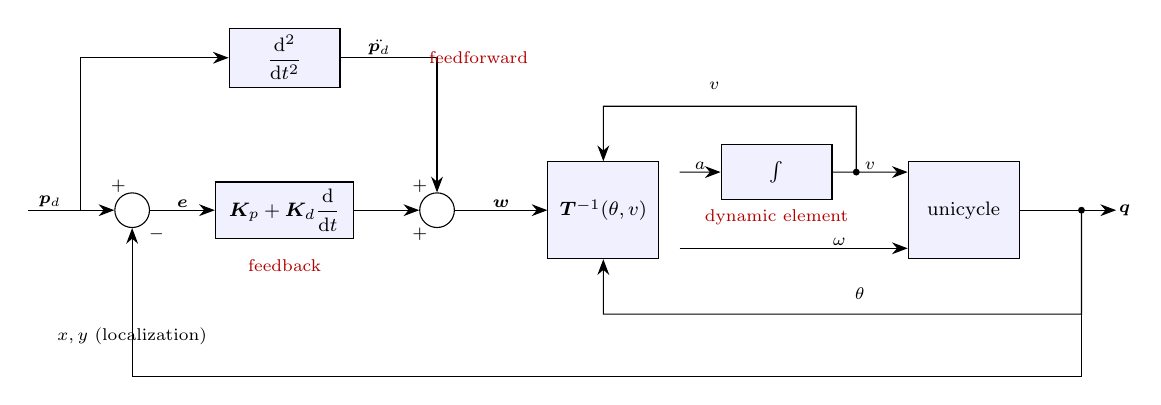
\begin{tikzpicture}[scale=0.88,transform shape]
\node[sm] (s1) at (0,0) {};
\node[blk,minimum width=20mm] (K) at (2.2,0) {$\vect K_p+\vect K_d\dfrac{\dd}{\dd t}$};
\node[sm] (s2) at (4.4,0) {};
\node[blk,minimum height=14mm] (T) at (6.8,0) {$\vect T^{-1}(\theta,v)$};
\node[blk] (int) at (9.3,0.55) {$\int$};
\node[blk,minimum height=14mm] (un) at (12.0,0) {unicycle};
\node[blk] (dd) at (2.2,2.2) {$\dfrac{\dd^2}{\dd t^2}$};
\draw[->] (-1.5,0) -- node[above,lab,pos=0.25]{$\pd$} (s1);
\draw[->] (-0.75,0) |- (dd.west);
\draw[->] (s1) -- node[above,lab]{$\vect e$} (K);
\draw[->] (K) -- (s2);
\draw[->] (dd.east) -| node[above,lab,pos=0.2]{$\ddot{\pd}$} (s2.north);
\draw[->] (s2) -- node[above,lab]{$\vect w$} (T);
\draw[->] (7.9,0.55) -- node[above,lab]{$a$} (int);
\draw[->] (int) -- node[above,lab]{$v$} (un.west |- 0,0.55);
\draw[->] (7.9,-0.55) -- node[above,lab,pos=0.7]{$\omega$} (un.west |- 0,-0.55);
\draw[->] (un) -- (14.2,0) node[right,lab]{$\vect q$};
\draw[->] (10.45,0.55) -- (10.45,1.5) -- (6.8,1.5) -- (T.north);
\node[dot] at (10.45,0.55) {};
\node[lab] at (8.4,1.8) {$v$};
\draw[->] (13.7,0) -- (13.7,-1.5) -- (6.8,-1.5) -- (T.south);
\node[dot] at (13.7,0) {};
\node[lab] at (10.5,-1.2) {$\theta$};
\draw[->] (13.7,-1.5) -- (13.7,-2.4) -- (0,-2.4) -- node[lab,pos=0.35,below]{$x,y$ (localization)} (s1.south);
\node[lab] at (-0.2,0.35) {$+$}; \node[lab] at (0.35,-0.35) {$-$};
\node[lab] at (4.15,0.35) {$+$}; \node[lab] at (4.15,-0.35) {$+$};
\node[lab,red!70!black] at (5.0,2.2) {feedforward};
\node[lab,red!70!black] at (2.2,-0.8) {feedback};
\node[lab,red!70!black] at (9.3,-0.1) {dynamic element};
\end{tikzpicture}
\caption{Tracking via output error feedback + dynamic i/o linearization: a \emph{dynamic} controller based on the output error; it needs $\dot{\pd}$ and $\ddot{\pd}$ (inside $\vect K_d$ and the feedforward), $(x,y)$ for the error and $\theta$ for the input transformation. The state $v$ of the integrator is fed back to $\vect T^{-1}$.}
\label{fig:dynamic_scheme}
\end{figure}

\begin{algorithm}[Dynamic i/o linearization tracker]
Initialize $v(0)\neq0$ (e.g.\ $v(0)=\vd(0)$). At each instant:
\begin{enumerate}[nosep]
\item compute $w_1,w_2$ as above (with $\dot x=v\cos\theta$, $\dot y=v\sin\theta$);
\item $a=\cos\theta\,w_1+\sin\theta\,w_2$, $\ \omega=(-\sin\theta\,w_1+\cos\theta\,w_2)/v$;
\item integrate $\dot v=a$ and send $(v,\omega)$ to the robot.
\end{enumerate}
\end{algorithm}

\begin{intuition}
Compared with the static scheme, we pay with extra machinery (one integrator, second derivatives of the reference, $v\neq0$) but we get the real thing: the point that converges is the actual position $(x,y)$, with zero steady-state error and no hidden heading dynamics. Static feedback tracks a \emph{fictitious} point $B$; dynamic feedback tracks the \emph{true} point.
\end{intuition}

%=====================================================================
\section{Simulations \texorpdfstring{\emph{(slides 29--40)}}{(slides 29--40)}}
%=====================================================================

The slides compare the three controllers on three reference trajectories: a circle, a square (with sharp corners) and a figure-8. The qualitative findings can be summarized as follows.

\begin{table}[H]
\centering\small
\begin{tabularx}{\textwidth}{@{}l>{\raggedright\arraybackslash}X>{\raggedright\arraybackslash}X>{\raggedright\arraybackslash}X@{}}
\toprule
 & \textbf{Approx.\ linearization} & \textbf{Static i/o lin.} ($b=0.75$ / $0.2$) & \textbf{Dynamic i/o lin.}\\
\midrule
Circle & converges; only local stability guaranteed & steady-state error $=b$; reducing $b$ lowers the error but \emph{increases steering velocity} & zero steady-state error, reasonable velocities\\
Square & only local stability; \emph{a new transient at each corner} & error $=b$; the displaced output gives a \emph{lookahead} behaviour (corners are cut); small $b$: smaller error, larger steering peaks & faster transients, reasonable velocities\\
Figure 8 & local stability not guaranteed (persistent $\vd,\omd$ vary), but good performance & error $=b$; smaller $b$ $\Rightarrow$ larger steering velocity & zero steady-state error, reasonable velocities\\
\bottomrule
\end{tabularx}
\caption{Qualitative outcome of the simulations.}
\end{table}

Reading off the circle plots, the \emph{initial} steering velocity grows from about $2.7$ rad/s for $b=0.75$ to about $10$ rad/s for $b=0.2$: a ratio $\approx 3.7\approx 0.75/0.2$, as expected from the $1/b$ factor in~\eqref{eq:Tinv}.

\begin{figure}[H]
\centering
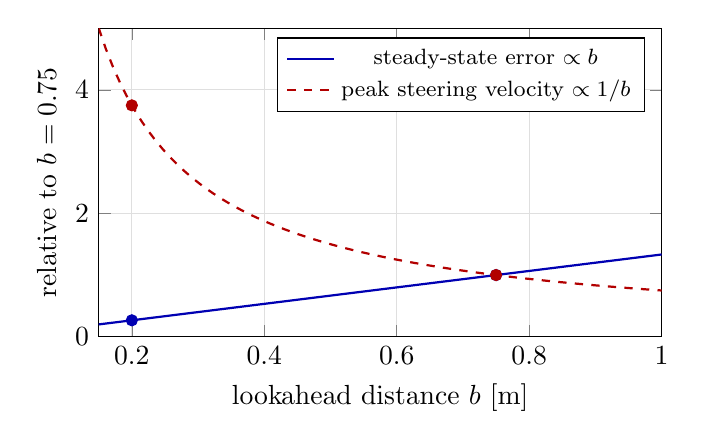
\begin{tikzpicture}
\begin{axis}[width=0.72\textwidth,height=5.5cm,xlabel={lookahead distance $b$ [m]},ylabel={relative to $b=0.75$},
  xmin=0.15,xmax=1.0,ymin=0,ymax=5,domain=0.15:1.0,samples=80,legend pos=north east,legend style={font=\footnotesize},grid=both,grid style={gray!25}]
\addplot[thick,blue!70!black]{x/0.75};
\addlegendentry{steady-state error $\propto b$}
\addplot[thick,red!70!black,dashed]{0.75/x};
\addlegendentry{peak steering velocity $\propto 1/b$}
\addplot[only marks,mark=*,blue!70!black] coordinates {(0.75,1) (0.2,0.2667)};
\addplot[only marks,mark=*,red!70!black] coordinates {(0.75,1) (0.2,3.75)};
\end{axis}
\end{tikzpicture}
\caption{The trade-off of static i/o linearization (original illustration of the scaling laws; the dots mark the two cases simulated, $b=0.75$ and $b=0.2$). A small $b$ gives small error but demands large steering velocities.}
\label{fig:tradeoff}
\end{figure}

\begin{example}[Circle tracking, independent simulation]
To visualize the comparison we simulated (Euler, $dt=2$~ms) the tracking of a circle of radius $3$~m with $\vd=1$~m/s ($\omd=1/3$~rad/s), starting from $\vect q(0)=(1,-1,2)$ and, for the dynamic controller, $v(0)=1.5$~m/s. Gains: approximate linearization $a=2,\zeta=0.7$; static i/o $k_x=k_y=2.5$; dynamic i/o $k_p=6.25$, $k_d=5$. Fig.~\ref{fig:sim} shows the paths and the error norm.
\end{example}

\begin{figure}[H]
\centering
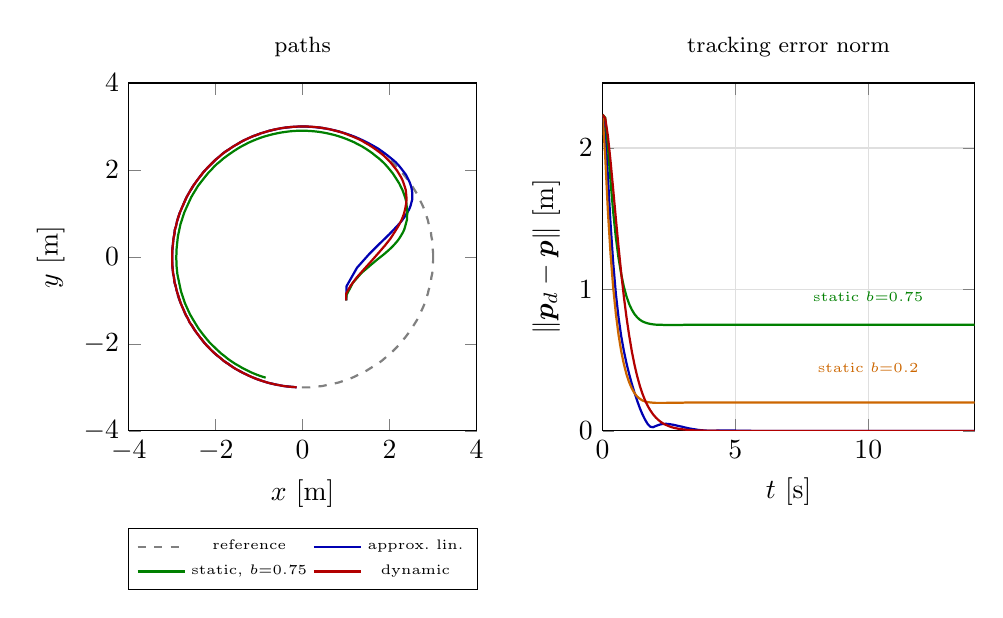
\begin{tikzpicture}
\begin{groupplot}[group style={group size=2 by 1,horizontal sep=1.6cm},width=0.52\textwidth,height=6cm]
\nextgroupplot[xlabel={$x$ [m]},ylabel={$y$ [m]},axis equal image,title={\footnotesize paths},legend style={font=\tiny,at={(0.5,-0.28)},anchor=north,legend columns=2},xmin=-4,xmax=4,ymin=-4,ymax=4]
\addplot[gray,thick,dashed] coordinates {(3.00,0.00) (3.00,0.09) (2.99,0.19) (2.99,0.28) (2.98,0.38) (2.96,0.47) (2.95,0.56) (2.93,0.66) (2.90,0.75) (2.88,0.84) (2.85,0.93) (2.82,1.02) (2.79,1.11) (2.75,1.20) (2.71,1.28) (2.67,1.37) (2.63,1.45) (2.58,1.53) (2.53,1.61) (2.48,1.69) (2.42,1.77) (2.36,1.85) (2.30,1.92) (2.24,1.99) (2.18,2.06) (2.11,2.13) (2.04,2.20) (1.97,2.26) (1.90,2.32) (1.83,2.38) (1.75,2.44) (1.67,2.49) (1.59,2.54) (1.51,2.59) (1.43,2.64) (1.35,2.68) (1.26,2.72) (1.18,2.76) (1.09,2.80) (1.00,2.83) (0.91,2.86) (0.82,2.89) (0.73,2.91) (0.63,2.93) (0.54,2.95) (0.45,2.97) (0.35,2.98) (0.26,2.99) (0.17,3.00) (0.07,3.00) (-0.02,3.00) (-0.12,3.00) (-0.21,2.99) (-0.31,2.98) (-0.40,2.97) (-0.49,2.96) (-0.59,2.94) (-0.68,2.92) (-0.77,2.90) (-0.86,2.87) (-0.95,2.84) (-1.04,2.81) (-1.13,2.78) (-1.22,2.74) (-1.30,2.70) (-1.39,2.66) (-1.47,2.61) (-1.55,2.57) (-1.63,2.52) (-1.71,2.46) (-1.79,2.41) (-1.87,2.35) (-1.94,2.29) (-2.01,2.23) (-2.08,2.16) (-2.15,2.10) (-2.21,2.03) (-2.27,1.96) (-2.33,1.88) (-2.39,1.81) (-2.45,1.73) (-2.50,1.65) (-2.55,1.57) (-2.60,1.49) (-2.65,1.41) (-2.69,1.33) (-2.73,1.24) (-2.77,1.15) (-2.80,1.07) (-2.84,0.98) (-2.87,0.89) (-2.89,0.80) (-2.92,0.70) (-2.94,0.61) (-2.95,0.52) (-2.97,0.42) (-2.98,0.33) (-2.99,0.24) (-3.00,0.14) (-3.00,0.05) (-3.00,-0.05) (-3.00,-0.14) (-2.99,-0.24) (-2.98,-0.33) (-2.97,-0.42) (-2.95,-0.52) (-2.94,-0.61) (-2.92,-0.70) (-2.89,-0.80) (-2.87,-0.89) (-2.84,-0.98) (-2.80,-1.07) (-2.77,-1.15) (-2.73,-1.24) (-2.69,-1.33) (-2.65,-1.41) (-2.60,-1.49) (-2.55,-1.57) (-2.50,-1.65) (-2.45,-1.73) (-2.39,-1.81) (-2.33,-1.88) (-2.27,-1.96) (-2.21,-2.03) (-2.15,-2.10) (-2.08,-2.16) (-2.01,-2.23) (-1.94,-2.29) (-1.87,-2.35) (-1.79,-2.41) (-1.71,-2.46) (-1.63,-2.52) (-1.55,-2.57) (-1.47,-2.61) (-1.39,-2.66) (-1.30,-2.70) (-1.22,-2.74) (-1.13,-2.78) (-1.04,-2.81) (-0.95,-2.84) (-0.86,-2.87) (-0.77,-2.90) (-0.68,-2.92) (-0.59,-2.94) (-0.49,-2.96) (-0.40,-2.97) (-0.31,-2.98) (-0.21,-2.99) (-0.12,-3.00) (-0.02,-3.00) (0.07,-3.00) (0.17,-3.00) (0.26,-2.99) (0.35,-2.98) (0.45,-2.97) (0.54,-2.95) (0.63,-2.93) (0.73,-2.91) (0.82,-2.89) (0.91,-2.86) (1.00,-2.83) (1.09,-2.80) (1.18,-2.76) (1.26,-2.72) (1.35,-2.68) (1.43,-2.64) (1.51,-2.59) (1.59,-2.54) (1.67,-2.49) (1.75,-2.44) (1.83,-2.38) (1.90,-2.32) (1.97,-2.26) (2.04,-2.20) (2.11,-2.13) (2.18,-2.06) (2.24,-1.99) (2.30,-1.92) (2.36,-1.85) (2.42,-1.77) (2.48,-1.69) (2.53,-1.61) (2.58,-1.53) (2.63,-1.45) (2.67,-1.37) (2.71,-1.28) (2.75,-1.20) (2.79,-1.11) (2.82,-1.02) (2.85,-0.93) (2.88,-0.84) (2.90,-0.75) (2.93,-0.66) (2.95,-0.56) (2.96,-0.47) (2.98,-0.38) (2.99,-0.28) (2.99,-0.19) (3.00,-0.09) (3.00,-0.00)};
\addlegendentry{reference}
\addplot[blue!70!black,thick] coordinates {(1.00,-1.000) (1.01,-0.672) (1.25,-0.249) (1.54,0.077) (1.79,0.324) (1.99,0.518) (2.14,0.675) (2.26,0.805) (2.34,0.915) (2.40,1.010) (2.45,1.095) (2.48,1.173) (2.50,1.247) (2.52,1.321) (2.52,1.396) (2.52,1.474) (2.51,1.554) (2.49,1.635) (2.46,1.718) (2.42,1.801) (2.38,1.883) (2.32,1.963) (2.26,2.041) (2.20,2.115) (2.13,2.187) (2.05,2.254) (1.97,2.319) (1.89,2.381) (1.81,2.439) (1.73,2.494) (1.64,2.546) (1.55,2.596) (1.46,2.643) (1.37,2.687) (1.28,2.728) (1.19,2.766) (1.09,2.802) (1.00,2.835) (0.90,2.865) (0.80,2.892) (0.71,2.916) (0.61,2.937) (0.51,2.955) (0.41,2.970) (0.31,2.982) (0.21,2.990) (0.11,2.996) (0.01,2.998) (-0.09,2.997) (-0.19,2.993) (-0.29,2.985) (-0.39,2.974) (-0.49,2.959) (-0.58,2.942) (-0.68,2.921) (-0.78,2.897) (-0.87,2.869) (-0.97,2.839) (-1.06,2.805) (-1.16,2.768) (-1.25,2.728) (-1.34,2.685) (-1.43,2.639) (-1.51,2.590) (-1.60,2.538) (-1.68,2.483) (-1.77,2.426) (-1.85,2.366) (-1.92,2.303) (-2.00,2.237) (-2.07,2.170) (-2.14,2.099) (-2.21,2.027) (-2.28,1.952) (-2.34,1.875) (-2.40,1.796) (-2.46,1.714) (-2.52,1.631) (-2.57,1.547) (-2.62,1.460) (-2.67,1.372) (-2.71,1.282) (-2.75,1.191) (-2.79,1.099) (-2.83,1.005) (-2.86,0.910) (-2.89,0.815) (-2.91,0.718) (-2.94,0.620) (-2.95,0.522) (-2.97,0.423) (-2.98,0.324) (-2.99,0.225) (-3.00,0.125) (-3.00,0.025) (-3.00,-0.075) (-3.00,-0.175) (-2.99,-0.275) (-2.98,-0.374) (-2.96,-0.473) (-2.95,-0.572) (-2.92,-0.670) (-2.90,-0.767) (-2.87,-0.863) (-2.84,-0.958) (-2.81,-1.052) (-2.77,-1.145) (-2.73,-1.237) (-2.69,-1.328) (-2.64,-1.417) (-2.60,-1.504) (-2.54,-1.590) (-2.49,-1.673) (-2.43,-1.756) (-2.37,-1.836) (-2.31,-1.914) (-2.25,-1.990) (-2.18,-2.063) (-2.11,-2.135) (-2.04,-2.204) (-1.96,-2.271) (-1.88,-2.335) (-1.81,-2.396) (-1.72,-2.455) (-1.64,-2.511) (-1.56,-2.564) (-1.47,-2.615) (-1.38,-2.663) (-1.29,-2.707) (-1.20,-2.749) (-1.11,-2.787) (-1.02,-2.823) (-0.92,-2.855) (-0.83,-2.884) (-0.73,-2.910) (-0.63,-2.933) (-0.53,-2.952) (-0.44,-2.968) (-0.34,-2.981) (-0.24,-2.991) (-0.14,-2.997)};
\addlegendentry{approx.\ lin.}
\addplot[green!50!black,thick] coordinates {(1.00,-1.000) (1.01,-0.877) (1.15,-0.601) (1.35,-0.372) (1.55,-0.200) (1.71,-0.065) (1.85,0.045) (1.96,0.139) (2.05,0.222) (2.12,0.297) (2.18,0.367) (2.23,0.436) (2.27,0.503) (2.31,0.571) (2.34,0.640) (2.36,0.712) (2.38,0.786) (2.40,0.863) (2.40,0.942) (2.41,1.023) (2.40,1.105) (2.39,1.189) (2.38,1.274) (2.36,1.358) (2.33,1.443) (2.30,1.526) (2.26,1.609) (2.22,1.691) (2.17,1.770) (2.12,1.848) (2.07,1.924) (2.01,1.998) (1.95,2.070) (1.89,2.138) (1.82,2.205) (1.75,2.268) (1.67,2.329) (1.60,2.387) (1.52,2.442) (1.44,2.495) (1.36,2.544) (1.27,2.590) (1.19,2.633) (1.10,2.673) (1.01,2.710) (0.92,2.744) (0.83,2.774) (0.74,2.801) (0.64,2.825) (0.55,2.846) (0.45,2.864) (0.36,2.878) (0.26,2.889) (0.16,2.896) (0.07,2.901) (-0.03,2.902) (-0.13,2.900) (-0.22,2.894) (-0.32,2.885) (-0.41,2.873) (-0.51,2.858) (-0.60,2.840) (-0.70,2.818) (-0.79,2.794) (-0.89,2.766) (-0.98,2.735) (-1.07,2.701) (-1.16,2.664) (-1.25,2.624) (-1.33,2.581) (-1.42,2.535) (-1.50,2.487) (-1.58,2.435) (-1.66,2.381) (-1.74,2.324) (-1.82,2.265) (-1.89,2.203) (-1.97,2.139) (-2.04,2.072) (-2.10,2.003) (-2.17,1.932) (-2.23,1.859) (-2.29,1.783) (-2.35,1.706) (-2.41,1.627) (-2.46,1.545) (-2.51,1.463) (-2.56,1.378) (-2.60,1.292) (-2.64,1.205) (-2.68,1.116) (-2.72,1.026) (-2.75,0.935) (-2.78,0.843) (-2.81,0.750) (-2.83,0.655) (-2.85,0.561) (-2.87,0.466) (-2.88,0.370) (-2.89,0.274) (-2.90,0.177) (-2.90,0.080) (-2.91,-0.017) (-2.90,-0.113) (-2.90,-0.210) (-2.89,-0.307) (-2.88,-0.403) (-2.86,-0.498) (-2.84,-0.593) (-2.82,-0.688) (-2.80,-0.782) (-2.77,-0.874) (-2.74,-0.966) (-2.71,-1.057) (-2.67,-1.147) (-2.63,-1.235) (-2.59,-1.322) (-2.54,-1.407) (-2.49,-1.491) (-2.44,-1.573) (-2.39,-1.654) (-2.33,-1.733) (-2.27,-1.810) (-2.21,-1.884) (-2.15,-1.957) (-2.08,-2.027) (-2.01,-2.095) (-1.94,-2.161) (-1.87,-2.225) (-1.79,-2.286) (-1.72,-2.344) (-1.64,-2.400) (-1.56,-2.454) (-1.47,-2.504) (-1.39,-2.552) (-1.30,-2.597) (-1.22,-2.639) (-1.13,-2.678) (-1.04,-2.714) (-0.95,-2.747) (-0.85,-2.777)};
\addlegendentry{static, $b{=}0.75$}
\addplot[red!70!black,thick] coordinates {(1.00,-1.000) (1.00,-0.846) (1.10,-0.667) (1.24,-0.477) (1.41,-0.285) (1.58,-0.096) (1.74,0.086) (1.89,0.259) (2.02,0.423) (2.12,0.578) (2.21,0.724) (2.28,0.861) (2.33,0.991) (2.36,1.113) (2.38,1.229) (2.39,1.339) (2.38,1.444) (2.37,1.544) (2.34,1.640) (2.31,1.732) (2.27,1.820) (2.22,1.904) (2.17,1.985) (2.11,2.062) (2.05,2.137) (1.99,2.208) (1.92,2.277) (1.85,2.342) (1.77,2.405) (1.69,2.464) (1.61,2.521) (1.53,2.574) (1.44,2.624) (1.36,2.672) (1.27,2.716) (1.18,2.757) (1.08,2.795) (0.99,2.830) (0.90,2.862) (0.80,2.890) (0.70,2.916) (0.61,2.938) (0.51,2.956) (0.41,2.972) (0.31,2.984) (0.21,2.993) (0.11,2.998) (0.01,3.000) (-0.09,2.999) (-0.19,2.994) (-0.29,2.986) (-0.39,2.975) (-0.49,2.961) (-0.58,2.943) (-0.68,2.922) (-0.78,2.897) (-0.87,2.870) (-0.97,2.839) (-1.06,2.805) (-1.16,2.768) (-1.25,2.728) (-1.34,2.685) (-1.43,2.639) (-1.51,2.590) (-1.60,2.538) (-1.68,2.483) (-1.77,2.426) (-1.85,2.365) (-1.92,2.303) (-2.00,2.237) (-2.07,2.170) (-2.14,2.099) (-2.21,2.027) (-2.28,1.952) (-2.34,1.875) (-2.40,1.796) (-2.46,1.714) (-2.52,1.631) (-2.57,1.547) (-2.62,1.460) (-2.67,1.372) (-2.71,1.282) (-2.75,1.191) (-2.79,1.099) (-2.83,1.005) (-2.86,0.910) (-2.89,0.815) (-2.91,0.718) (-2.94,0.620) (-2.95,0.522) (-2.97,0.423) (-2.98,0.324) (-2.99,0.225) (-3.00,0.125) (-3.00,0.025) (-3.00,-0.075) (-3.00,-0.175) (-2.99,-0.275) (-2.98,-0.374) (-2.96,-0.473) (-2.95,-0.572) (-2.92,-0.669) (-2.90,-0.767) (-2.87,-0.863) (-2.84,-0.958) (-2.81,-1.052) (-2.77,-1.145) (-2.73,-1.237) (-2.69,-1.328) (-2.64,-1.417) (-2.60,-1.504) (-2.54,-1.590) (-2.49,-1.673) (-2.43,-1.756) (-2.37,-1.836) (-2.31,-1.914) (-2.25,-1.990) (-2.18,-2.063) (-2.11,-2.135) (-2.04,-2.204) (-1.96,-2.271) (-1.88,-2.335) (-1.81,-2.396) (-1.72,-2.455) (-1.64,-2.511) (-1.56,-2.564) (-1.47,-2.615) (-1.38,-2.663) (-1.29,-2.707) (-1.20,-2.749) (-1.11,-2.787) (-1.02,-2.823) (-0.92,-2.855) (-0.83,-2.884) (-0.73,-2.910) (-0.63,-2.933) (-0.53,-2.952) (-0.44,-2.969) (-0.34,-2.981) (-0.24,-2.991) (-0.14,-2.997)};
\addlegendentry{dynamic}
\nextgroupplot[xlabel={$t$ [s]},ylabel={$\|\pd-\vect p\|$ [m]},title={\footnotesize tracking error norm},xmin=0,xmax=14,ymin=0,grid=both,grid style={gray!25}]
\addplot[blue!70!black,thick] coordinates {(0.00,2.236) (0.10,2.128) (0.20,1.800) (0.30,1.465) (0.40,1.187) (0.50,0.970) (0.60,0.802) (0.70,0.671) (0.80,0.566) (0.90,0.478) (1.00,0.402) (1.10,0.333) (1.20,0.271) (1.30,0.214) (1.40,0.162) (1.50,0.117) (1.60,0.079) (1.70,0.048) (1.80,0.029) (1.90,0.026) (2.00,0.034) (2.10,0.041) (2.20,0.047) (2.30,0.049) (2.40,0.050) (2.50,0.048) (2.60,0.045) (2.70,0.042) (2.80,0.037) (2.90,0.033) (3.00,0.029) (3.10,0.024) (3.20,0.020) (3.30,0.016) (3.40,0.013) (3.50,0.010) (3.60,0.007) (3.70,0.005) (3.80,0.003) (3.90,0.002) (4.00,0.001) (4.10,0.001) (4.20,0.001) (4.30,0.002) (4.40,0.002) (4.50,0.002) (4.60,0.002) (4.70,0.002) (4.80,0.002) (4.90,0.002) (5.00,0.002) (5.10,0.001) (5.20,0.001) (5.30,0.001) (5.40,0.001) (5.50,0.001) (5.60,0.000) (5.70,0.000) (5.80,0.000) (5.90,0.000) (6.00,0.000) (6.10,0.000) (6.20,0.000) (6.30,0.000) (6.40,0.000) (6.50,0.000) (6.60,0.000) (6.70,0.000) (6.80,0.000) (6.90,0.000) (7.00,0.000) (7.10,0.000) (7.20,0.000) (7.30,0.000) (7.40,0.000) (7.50,0.000) (7.60,0.000) (7.70,0.000) (7.80,0.000) (7.90,0.000) (8.00,0.000) (8.10,0.000) (8.20,0.000) (8.30,0.000) (8.40,0.000) (8.50,0.000) (8.60,0.000) (8.70,0.000) (8.80,0.000) (8.90,0.000) (9.00,0.000) (9.10,0.000) (9.20,0.000) (9.30,0.000) (9.40,0.000) (9.50,0.000) (9.60,0.000) (9.70,0.000) (9.80,0.000) (9.90,0.000) (10.00,0.000) (10.10,0.000) (10.20,0.000) (10.30,0.000) (10.40,0.000) (10.50,0.000) (10.60,0.000) (10.70,0.000) (10.80,0.000) (10.90,0.000) (11.00,0.000) (11.10,0.000) (11.20,0.000) (11.30,0.000) (11.40,0.000) (11.50,0.000) (11.60,0.000) (11.70,0.000) (11.80,0.000) (11.90,0.000) (12.00,0.000) (12.10,0.000) (12.20,0.000) (12.30,0.000) (12.40,0.000) (12.50,0.000) (12.60,0.000) (12.70,0.000) (12.80,0.000) (12.90,0.000) (13.00,0.000) (13.10,0.000) (13.20,0.000) (13.30,0.000) (13.40,0.000) (13.50,0.000) (13.60,0.000) (13.70,0.000) (13.80,0.000) (13.90,0.000) (14.00,0.000)};
\addplot[green!50!black,thick] coordinates {(0.00,2.236) (0.10,2.214) (0.20,2.010) (0.30,1.764) (0.40,1.546) (0.50,1.366) (0.60,1.222) (0.70,1.109) (0.80,1.020) (0.90,0.951) (1.00,0.897) (1.10,0.857) (1.20,0.826) (1.30,0.803) (1.40,0.786) (1.50,0.774) (1.60,0.766) (1.70,0.760) (1.80,0.756) (1.90,0.753) (2.00,0.751) (2.10,0.750) (2.20,0.750) (2.30,0.749) (2.40,0.749) (2.50,0.749) (2.60,0.749) (2.70,0.749) (2.80,0.749) (2.90,0.749) (3.00,0.749) (3.10,0.750) (3.20,0.750) (3.30,0.750) (3.40,0.750) (3.50,0.750) (3.60,0.750) (3.70,0.750) (3.80,0.750) (3.90,0.750) (4.00,0.750) (4.10,0.750) (4.20,0.750) (4.30,0.750) (4.40,0.750) (4.50,0.750) (4.60,0.750) (4.70,0.750) (4.80,0.750) (4.90,0.750) (5.00,0.750) (5.10,0.750) (5.20,0.750) (5.30,0.750) (5.40,0.750) (5.50,0.750) (5.60,0.750) (5.70,0.750) (5.80,0.750) (5.90,0.750) (6.00,0.750) (6.10,0.750) (6.20,0.750) (6.30,0.750) (6.40,0.750) (6.50,0.750) (6.60,0.750) (6.70,0.750) (6.80,0.750) (6.90,0.750) (7.00,0.750) (7.10,0.750) (7.20,0.750) (7.30,0.750) (7.40,0.750) (7.50,0.750) (7.60,0.750) (7.70,0.750) (7.80,0.750) (7.90,0.750) (8.00,0.750) (8.10,0.750) (8.20,0.750) (8.30,0.750) (8.40,0.750) (8.50,0.750) (8.60,0.750) (8.70,0.750) (8.80,0.750) (8.90,0.750) (9.00,0.750) (9.10,0.750) (9.20,0.750) (9.30,0.750) (9.40,0.750) (9.50,0.750) (9.60,0.750) (9.70,0.750) (9.80,0.750) (9.90,0.750) (10.00,0.750) (10.10,0.750) (10.20,0.750) (10.30,0.750) (10.40,0.750) (10.50,0.750) (10.60,0.750) (10.70,0.750) (10.80,0.750) (10.90,0.750) (11.00,0.750) (11.10,0.750) (11.20,0.750) (11.30,0.750) (11.40,0.750) (11.50,0.750) (11.60,0.750) (11.70,0.750) (11.80,0.750) (11.90,0.750) (12.00,0.750) (12.10,0.750) (12.20,0.750) (12.30,0.750) (12.40,0.750) (12.50,0.750) (12.60,0.750) (12.70,0.750) (12.80,0.750) (12.90,0.750) (13.00,0.750) (13.10,0.750) (13.20,0.750) (13.30,0.750) (13.40,0.750) (13.50,0.750) (13.60,0.750) (13.70,0.750) (13.80,0.750) (13.90,0.750) (14.00,0.750)};
\addplot[orange!80!black,thick] coordinates {(0.00,2.236) (0.10,1.936) (0.20,1.552) (0.30,1.250) (0.40,1.012) (0.50,0.827) (0.60,0.680) (0.70,0.564) (0.80,0.473) (0.90,0.400) (1.00,0.344) (1.10,0.300) (1.20,0.267) (1.30,0.243) (1.40,0.227) (1.50,0.215) (1.60,0.208) (1.70,0.203) (1.80,0.201) (1.90,0.199) (2.00,0.198) (2.10,0.198) (2.20,0.198) (2.30,0.198) (2.40,0.198) (2.50,0.199) (2.60,0.199) (2.70,0.199) (2.80,0.199) (2.90,0.199) (3.00,0.199) (3.10,0.200) (3.20,0.200) (3.30,0.200) (3.40,0.200) (3.50,0.200) (3.60,0.200) (3.70,0.200) (3.80,0.200) (3.90,0.200) (4.00,0.200) (4.10,0.200) (4.20,0.200) (4.30,0.200) (4.40,0.200) (4.50,0.200) (4.60,0.200) (4.70,0.200) (4.80,0.200) (4.90,0.200) (5.00,0.200) (5.10,0.200) (5.20,0.200) (5.30,0.200) (5.40,0.200) (5.50,0.200) (5.60,0.200) (5.70,0.200) (5.80,0.200) (5.90,0.200) (6.00,0.200) (6.10,0.200) (6.20,0.200) (6.30,0.200) (6.40,0.200) (6.50,0.200) (6.60,0.200) (6.70,0.200) (6.80,0.200) (6.90,0.200) (7.00,0.200) (7.10,0.200) (7.20,0.200) (7.30,0.200) (7.40,0.200) (7.50,0.200) (7.60,0.200) (7.70,0.200) (7.80,0.200) (7.90,0.200) (8.00,0.200) (8.10,0.200) (8.20,0.200) (8.30,0.200) (8.40,0.200) (8.50,0.200) (8.60,0.200) (8.70,0.200) (8.80,0.200) (8.90,0.200) (9.00,0.200) (9.10,0.200) (9.20,0.200) (9.30,0.200) (9.40,0.200) (9.50,0.200) (9.60,0.200) (9.70,0.200) (9.80,0.200) (9.90,0.200) (10.00,0.200) (10.10,0.200) (10.20,0.200) (10.30,0.200) (10.40,0.200) (10.50,0.200) (10.60,0.200) (10.70,0.200) (10.80,0.200) (10.90,0.200) (11.00,0.200) (11.10,0.200) (11.20,0.200) (11.30,0.200) (11.40,0.200) (11.50,0.200) (11.60,0.200) (11.70,0.200) (11.80,0.200) (11.90,0.200) (12.00,0.200) (12.10,0.200) (12.20,0.200) (12.30,0.200) (12.40,0.200) (12.50,0.200) (12.60,0.200) (12.70,0.200) (12.80,0.200) (12.90,0.200) (13.00,0.200) (13.10,0.200) (13.20,0.200) (13.30,0.200) (13.40,0.200) (13.50,0.200) (13.60,0.200) (13.70,0.200) (13.80,0.200) (13.90,0.200) (14.00,0.200)};
\addplot[red!70!black,thick] coordinates {(0.00,2.236) (0.10,2.209) (0.20,2.085) (0.30,1.907) (0.40,1.706) (0.50,1.500) (0.60,1.302) (0.70,1.118) (0.80,0.951) (0.90,0.803) (1.00,0.675) (1.10,0.563) (1.20,0.468) (1.30,0.388) (1.40,0.320) (1.50,0.263) (1.60,0.215) (1.70,0.176) (1.80,0.144) (1.90,0.117) (2.00,0.095) (2.10,0.077) (2.20,0.062) (2.30,0.050) (2.40,0.041) (2.50,0.033) (2.60,0.026) (2.70,0.021) (2.80,0.017) (2.90,0.013) (3.00,0.011) (3.10,0.009) (3.20,0.007) (3.30,0.005) (3.40,0.004) (3.50,0.003) (3.60,0.003) (3.70,0.002) (3.80,0.002) (3.90,0.001) (4.00,0.001) (4.10,0.001) (4.20,0.001) (4.30,0.001) (4.40,0.000) (4.50,0.000) (4.60,0.000) (4.70,0.000) (4.80,0.000) (4.90,0.000) (5.00,0.000) (5.10,0.000) (5.20,0.000) (5.30,0.000) (5.40,0.000) (5.50,0.000) (5.60,0.000) (5.70,0.000) (5.80,0.000) (5.90,0.000) (6.00,0.000) (6.10,0.000) (6.20,0.000) (6.30,0.000) (6.40,0.000) (6.50,0.000) (6.60,0.000) (6.70,0.000) (6.80,0.000) (6.90,0.000) (7.00,0.000) (7.10,0.000) (7.20,0.000) (7.30,0.000) (7.40,0.000) (7.50,0.000) (7.60,0.000) (7.70,0.000) (7.80,0.000) (7.90,0.000) (8.00,0.000) (8.10,0.000) (8.20,0.000) (8.30,0.000) (8.40,0.000) (8.50,0.000) (8.60,0.000) (8.70,0.000) (8.80,0.000) (8.90,0.000) (9.00,0.000) (9.10,0.000) (9.20,0.000) (9.30,0.000) (9.40,0.000) (9.50,0.000) (9.60,0.000) (9.70,0.000) (9.80,0.000) (9.90,0.000) (10.00,0.000) (10.10,0.000) (10.20,0.000) (10.30,0.000) (10.40,0.000) (10.50,0.000) (10.60,0.000) (10.70,0.000) (10.80,0.000) (10.90,0.000) (11.00,0.000) (11.10,0.000) (11.20,0.000) (11.30,0.000) (11.40,0.000) (11.50,0.000) (11.60,0.000) (11.70,0.000) (11.80,0.000) (11.90,0.000) (12.00,0.000) (12.10,0.000) (12.20,0.000) (12.30,0.000) (12.40,0.000) (12.50,0.000) (12.60,0.000) (12.70,0.000) (12.80,0.000) (12.90,0.000) (13.00,0.000) (13.10,0.000) (13.20,0.000) (13.30,0.000) (13.40,0.000) (13.50,0.000) (13.60,0.000) (13.70,0.000) (13.80,0.000) (13.90,0.000) (14.00,0.000)};
\node[font=\tiny,green!50!black] at (axis cs:10,0.95) {static $b{=}0.75$};
\node[font=\tiny,orange!80!black] at (axis cs:10,0.45) {static $b{=}0.2$};
\end{groupplot}
\end{tikzpicture}
\caption{Original simulation of the three controllers on a circle. Approximate linearization and dynamic i/o linearization converge to zero error; static i/o linearization settles at an error equal to $b$.}
\label{fig:sim}
\end{figure}

%=====================================================================
\section{Summary}
%=====================================================================

\begin{table}[H]
\centering\footnotesize
\setlength{\tabcolsep}{4pt}
\begin{tabularx}{\textwidth}{@{}>{\raggedright\arraybackslash}p{2.35cm}>{\raggedright\arraybackslash}X>{\raggedright\arraybackslash}X>{\raggedright\arraybackslash}X@{}}
\toprule
 & \textbf{State error + approx.\ linearization} & \textbf{Output error + static i/o lin.} & \textbf{Output error + dynamic i/o lin.}\\
\midrule
Controlled variable & state error $\vect e=\vect R(\theta)(\qd-\vect q)$ & Cartesian position of $B$ (displaced by $b$) & Cartesian position $(x,y)$\\
Controller type & static & static & dynamic (integrator on $v$)\\
Reference needed & $\vd,\omd$ (and $\theta_d$) via flatness & $\pd,\dot{\pd}$ & $\pd,\dot{\pd},\ddot{\pd}$\\
Measurements & $x,y,\theta$ & $x,y,\theta$ & $x,y,\theta$ (and $v$ internal)\\
Stability & local, only for constant $\vd,\omd$ (global with nonlinear version) & global exponential for $B$ & global exponential for $(x,y)$\\
Zero dynamics & none ($\theta$ in the error) & yes: $\theta$ aligns with motion (forward only) & none\\
Steady-state error & $0$ & $b$ (contact point) & $0$\\
Restrictions & persistent trajectory ($k_2\to\infty$ as $\vd\to0$); smooth direction & none on corners; $b\neq0$; large $\omega$ if $b$ small & persistent ($v\neq0$); trajectory twice differentiable\\
\bottomrule
\end{tabularx}
\caption{Comparison of the trajectory tracking controllers for the unicycle.}
\end{table}

\begin{intuition}
Pick the tool by what you can accept. \emph{State error + linearization}: simplest idea, but the guarantees are weak. \emph{Static i/o}: guaranteed and simple, but you pay with a permanent offset $b$ (a lookahead, which is sometimes even desirable on corners). \emph{Dynamic i/o}: the ``right'' answer (true position, zero error, globally exponentially stable) at the cost of more machinery and a ban on stopping. The trade-off between offset and steering effort in the static case is shown again in Fig.~\ref{fig:tradeoff}.
\end{intuition}

\subsection*{Key take-aways}
\begin{enumerate}
\item WMR motion control is designed on the \emph{kinematic} model, since the fast low-level loops let us treat velocities as inputs; reference inputs must always be applied together with a feedback correction.
\item For an admissible Cartesian trajectory, \emph{flatness} gives $\theta_d,\vd,\omd$ algebraically, and the nominal inputs act as feedforward in all schemes.
\item State error feedback with approximate linearization has a time-varying closed loop: pole placement with $k_2=(a^2-\omd^2)/\vd$ is only rigorous for circles and lines (local stability), and requires $\vd\neq0$; a nonlinear variant gives global stability.
\item Exact i/o linearization of $(x,y)$ fails with static feedback (singular decoupling matrix); displacing the output to $B$ at distance $b$ fixes this, at the cost of a zero dynamics and a steady-state error $b$ with steering velocity $\propto1/b$.
\item A dynamic extension ($\dot v=a$) allows tracking the true flat output $(x,y)$ with global exponential convergence and zero steady-state error, but needs a twice-differentiable, persistent trajectory ($v\neq0$, a structural limitation of nonholonomic systems).
\end{enumerate}

\end{document}